%%%%%%%%%%%%%%%%%%%%%%%%%%%%%%%%%%%%%%%%%%%%%%%%%%%%%%%%%%%%%%%%%%%%%%%%%%%%%%%%%%%%%%%%%%%%%%%%%%%%%%%%%%%%%%%%%%%%%%%%%%%%%
\section{Introduction}\label{sec:introduction}
The rapid advancement of artificial intelligence has enabled the generation of hyper-realistic audio deepfakes, which bring about severe risks to digital security and erode confidence in voice communications \cite{sahidullah2023introduction}. These speech outputs, generated by voice conversion and text-to-speech systems, have minimal perceptual artifacts, thus enabling malicious applications from financial fraud to political manipulation. Recent ASVspoof challenges \cite{wang2024asvspoof} have demonstrated an alarming trend where detection methods consistently fall behind the invention of sophisticated synthesis techniques, leaving considerable vulnerabilities in these systems. This ongoing arms race highlights the urgency to develop innovative detection systems that can successfully counteract emerging threats while ensuring operational efficiency on diverse platforms. Adding to these challenges, Rabhi et al. \cite{rabhi2024audio} have recently demonstrated that even state-of-the-art detectors are vulnerable to adversarial manipulation, highlighting the need to design architectures that are robust to both synthesized and manipulated inputs.

Existing detection techniques show promising results; however, they are faced with inherent limitations on their practical feasibility in real-life scenarios. Graph based systems like Aasist \cite{jung2022aasist} leverage unified spectro-temporal attention to evaluate multiple feature representations simultaneously, thus achieving benchmark performance without resorting to manual feature engineering. Concurrently, modifications of Wav2vec 2.0 \cite{martin2022vicomtech, tak2022automatic} incorporate self-supervised pretraining on large speech databases, showing improved generalizability to different classes of attacks through data augmentation strategies. WaveFake \cite{frank2021wavefake} has also improved evaluation techniques by incorporating a variety of generation methods, while Vicomtech's system \cite{martin2022vicomtech} combines Wav2vec2 embeddings with custom classifiers to identify synthetic artifacts. Yet, three key shortcomings persist: Firstly, there is a deterioration in performance when faced with new synthesis techniques not included in the training data, as reported by Li et al. \cite{li2024cross} in their cross dataset evaluations. Secondly, acoustic environmental variability and linguistic diversity negatively impact the consistency of detection, especially in low resource languages lacking large training datasets. Finally, the computational requirements present a formidable obstacle to deployment on resource constrained hardware, especially mobile platforms requiring real time processing this issue is further compounded by the growing reliance on voice authentication in handheld devices.

These limitations stem from two unresolved technical challenges in the field. First, the trade-off between detection accuracy and computational efficiency remains unaddressed, with transformer based architectures like Wav2vec2 demanding substantial processing power ill-suited for edge devices. Second, current frameworks lack adaptive mechanisms to counter adversarial attacks or zero-day synthesis techniques, relying instead on static training data that quickly becomes obsolete. Recent work by Farooq et al. \cite{farooq2025transferable} highlights the importance of dynamic model updating, yet their focus on text-based deepfakes leaves audio systems underserved.

The motivation for this research comes from the proven effectiveness of retrieval-augmented generation (RAG) in natural language processing (NLP) applications \cite{lewis2020retrieval}, demonstrating its potential in meeting current challenges related to audio deepfake detection. Traditional classification approaches rely on rigid decision boundaries that lose performance when faced with adaptive attack surfaces, while retrieval approaches provide dynamic access to validated speech samples. Additionally, voice profiles based on individual speakers can help reduce variability related issues by creating personalized detection thresholds rather than using standardized parameters. Integration with mobile technologies also offers practical advantages, such as increased computational efficiency and potential for effortless integration with traditional communication platforms. Recent work by Chen et al. \cite{chen2025wavrag} proves the efficacy of retrieval approaches in audio processing, attaining accuracy matching that of text based models while showing enhanced efficiency. Based on these findings, we propose a hybrid model that combines the flexibility of RAG with neural models optimized for on device inference.

This research work amplifies the effectiveness of deepfake detection through below main contributions: 
\begin{itemize}
    \item We introduce a retrieval-augmented framework for deepfake audio detection (RADAD) that retrieves nearest neighbor speech from a vector database and conditions the decision on this contextual evidence, strengthening discrimination.
    \item We extend a lightweight projection–fusion classifier (with temporal pyramid pooling) to operate inside the retrieval loop, enabling end-to-end training that jointly leverages query and neighborhood embeddings.
    \item Through extensive experiments on the Release-in-the-Wild benchmark, RADAD consistently outperforms strong baselines; the WavLM-RADAD variant achieves state-of-the-art EER with stable AUC gains, validating the effectiveness of retrieval based conditioning.
\end{itemize}

Cumulatively, these contributions are intended to bridge the gap between theoretical robustness and practical feasibility, thus providing a path towards adaptive defense systems that can counter next generation synthetic artifacts.

%%%%%%%%%%%%%%%%%%%%%%%%%%%%%%%%%%%%%%%%%%%%%%%%%%%%%%%%%%%%%%%%%%%%%%%%%%%%%%%%%%%%%%%%%%%%%%%%%%%%%%%%%%%%%%%%%%%%%%%%%%%%%
\section{Literature Review}\label{sec:literature_review}

The proliferation of AI generated synthetic speech poses increasing threats to media integrity and societal trust. This section examines the evolution of audio deepfake detection research, from foundational approaches to current state-of-the-art methods, with emphasis on retrieval-augmented frameworks and self-supervised feature extractors for non-text modalities.

\subsection{Foundations of Deepfake Audio Detection}\label{sec:literature_review:foundations}

Early research in deepfake audio identification relied on hand-crafted features including Mel-frequency cepstral coefficients (MFCC) \cite{hamza2022deepfake}, linear-frequency cepstral coefficients (LFCC) \cite{davis1980comparison}, \cite{luo2021capsule}, \cite{wang2021comparative}, and Constant-Q Transform (CQT) \cite{li2021channel}. However, these approaches exhibited limited effectiveness due to insufficient training data and inability to capture subtle synthesis artifacts across diverse acoustic conditions. As the field progressed, researchers transitioned from manual feature engineering to learned representations. Khochare et al. \cite{khochare2021deep} developed CNN based frameworks employing XceptionNet to automatically extract discriminative patterns from raw audio, substantially improving detection accuracy. This paradigm shift toward end-to-end learning enabled deep neural networks to discover hierarchical acoustic patterns without hand-crafted intermediaries, establishing the foundation for contemporary deepfake detection systems.

\subsection{Benchmarks and Evaluation Frameworks}\label{sec:literature_review:benchmarks}

Multiple benchmark datasets have proven instrumental in advancing audio deepfake detection. The ASVspoof challenge series \cite{wang2024asvspoof} (2019, 2021 editions) established standardized evaluation protocols for logical and physical access attacks. WaveFake \cite{frank2021wavefake} introduced high quality synthetic samples from multiple generators, while ADD 2022 \cite{yi2022add} expanded coverage to diverse attack types and recording conditions. Most recently, SONAR \cite{li2024sonar} emerged as a comprehensive framework evaluating both traditional and foundation model based systems. These benchmarks employ standard metrics including Equal Error Rate (EER), tandem Detection Cost Function (t-DCF), and minimum Detection Cost Function (min-DCF) for performance comparison.

\subsection{Recent Advancements in Deepfake Audio Detection}\label{sec:literature_review:advancements}

Contemporary approaches employ sophisticated architectures designed for enhanced discrimination. DeepSonar \cite{wang2020deepsonar} introduces neuron-level monitoring to distinguish acoustic characteristics between authentic and synthetic speech. The Aasist framework \cite{jung2022aasist} employs spectro-temporal graph attention networks, eliminating the need for hand-engineered features and enabling end-to-end learning from spectrograms. DST-Net \cite{ilyas2023avfakenet} combines dense temporal convolutions with attention mechanisms for multi-scale feature fusion. Additionally, XLS-R based systems \cite{zhang2024audio} leverage large-scale multilingual pretraining for acoustic representation learning, promoting robustness across diverse languages and recording conditions.

More recently, detector fusion strategies combining multiple feature extractors have emerged as promising directions. Kawa et al. \cite{kawa2023improved} demonstrated that integrating state-of-the-art speech recognition models with classical detection architectures (LCNN, SpecRNet, MesoNet) substantially enhances detection capability. MesoNet \cite{afchar2018mesonet}, a lightweight convolutional architecture, provides a practical baseline for resource constrained deployments. These architectures collectively demonstrate the effectiveness of combining strong feature representations with appropriate classification strategies.

\subsection{Self-Supervised Feature Extractors for Deepfake Detection}\label{sec:literature_review:extractors}

\subsubsection{Wav2Vec 2.0}

Wav2Vec 2.0 \cite{baevski2020wav2vec} pioneered self-supervised speech representation learning through masked prediction on unlabeled speech data. The model learns contextualized acoustic representations by predicting masked regions in a contrastive learning framework, trained on 960 hours of unlabeled LibriSpeech audio. Its key innovation lies in demonstrating that large unlabeled speech corpora can be effectively leveraged for downstream task learning without manual annotation. The primary advantage is superior performance on speech recognition and speaker verification tasks through effective transfer learning. However, limitations for deepfake detection include: (i) optimization objectives prioritize phonetic content over speaker identity, reducing discriminative power for speaker specific analysis; (ii) representations emphasize linguistic structure rather than synthesis artifact sensitivity; and (iii) limited speaker aware organization in the embedding space.

\subsubsection{WavLM}

WavLM (Wave Language Model) \cite{Chen_2022} extends Wav2Vec 2.0 by incorporating dual pretraining objectives: masked speech prediction combined with utterance mixing for speaker identification from mixed speech. Pretrained on 94,000 hours of multilingual audio across 53 languages, WavLM introduces speaker discriminative pretraining objectives specifically designed to preserve speaker identity in learned representations. The key innovation is dual-objective learning that simultaneously optimizes for both acoustic modeling and speaker discrimination. Primary advantages include: (i) inherent speaker awareness enabling natural clustering of same speaker utterances; (ii) robust multilingual pretraining promoting generalization across diverse languages and acoustic conditions; and (iii) simultaneous sensitivity to both natural speech characteristics and synthesis artifacts. Limitations include marginally higher computational requirements during inference and potential sensitivity to speaker variations that might impact content based analysis.

\subsubsection{Whisper}

Whisper \cite{radford2023robust} is a large-scale multilingual speech recognition model trained through weakly supervised learning on 680,000 hours of multilingual audio from diverse sources. Its key innovation is robust end-to-end speech-to-text conversion across 99 languages, trained without task specific labeling by leveraging diverse internet audio. The model produces rich representations capturing both acoustic properties and linguistic content. Primary advantages include: (i) massive exposure to diverse acoustic conditions, languages, and speaking styles during pretraining promoting robustness across varied data distributions; (ii) linguistic representations enabling content based consistency checking; and (iii) seamless integration into hybrid detection pipelines combining spectral and textual analysis. Limitations include: (i) optimization toward speech recognition rather than speaker discrimination, limiting speaker-identity preservation; (ii) substantial model size creating deployment challenges on resource constrained edge devices; and (iii) focus on linguistic correctness over acoustic artifact sensitivity.

The distinct design philosophies of these three extractors reflect different optimization objectives: Wav2Vec 2.0 prioritizes general acoustic modeling, WavLM specifically targets speaker discriminative learning, and Whisper emphasizes multilingual robustness for speech understanding. These differences have important implications for retrieval-augmented systems, where feature extractor choice fundamentally shapes whether retrieved neighbors reflect speaker similarity, content similarity, or linguistic consistency.

\subsection{RAG Applications on Non-Text Data}\label{sec:literature_review:rag}

Although the Retrieval Augmented Generation (RAG) framework \cite{lewis2020retrieval} has primarily been explored for text based NLP tasks, recent research has extended its application to multimodal data. Chen et al. \cite{chen2025wavrag} introduced WavRAG, a pioneering end-to-end audio RAG framework that processes raw audio directly without requiring Automatic Speech Recognition transcription. The key innovation is demonstrating that retrieval principles can be effectively adapted to audio modalities with substantial efficiency gains. Similar work by Jeong et al. \cite{jeong2025videorag} and Riedler et al. \cite{riedler2024beyond} demonstrated RAG framework utility across video and image modalities.

The application of retrieval-augmented techniques to deepfake audio detection has recently emerged as a promising research direction. Kang et al. \cite{Kang_2024} proposed the Retrieval-Augmented Detection (RAD) framework, representing the first comprehensive application of retrieval-augmented principles specifically to audio deepfake detection. RAD combines a retriever module with multi-fusion attentive classification, grounding detection decisions in neighborhoods of similar samples. The key innovation is leveraging retrieved neighbors predominantly from the same speaker for speaker specific discrimination. The framework demonstrates that instance level context can substantially enhance detection robustness.

However, RAD exhibits certain limitations motivating further research refinement. First, the framework maintains an external knowledge base exclusively from bonafide samples, leading to performance degradation in low-resource speaker scenarios. Second, time-wise compression operations introduce potential performance-accuracy trade-offs requiring careful calibration. Third, the dependency on comprehensive external reference databases limits scalability and practical deployment in diverse speaker environments. These limitations underscore the necessity for retrieval-augmented frameworks achieving more efficient multi-scale feature aggregation and reduced dependency on comprehensive external reference data.

To leverage RAG principles for audio, multiple feature extraction options exist. SentenceTransformers \cite{reimers2019sentence} combined with audio encoders enable unified embedding spaces for audio-text retrieval. Critically, feature extractor selection fundamentally impacts retrieval effectiveness: extractors optimized for speaker discrimination naturally produce embeddings where same speaker samples cluster coherently, while those emphasizing content produce different neighborhood structures. The synergy between feature extractor design and retrieval based detection architecture remains an important research dimension.

\subsection{Related Detection Architectures and Comparative Systems}\label{sec:literature_review:related}

Several contemporary architectures serve as important points of reference for deepfake detection. The AASIST framework \cite{jung2022aasist} introduces graph attention mechanisms for multi-scale spectro-temporal feature fusion, eliminating hand-engineered features entirely. DST-Net \cite{ilyas2023avfakenet} combines dense temporal convolutions with spatial attention for capturing both temporal and channel-wise dependencies. Kawa et al. \cite{kawa2023improved} demonstrated the effectiveness of combining modern foundation models (Whisper) with classical detection architectures, showing that strong feature extractors complement well designed classifiers. MesoNet \cite{afchar2018mesonet}, a lightweight convolutional architecture, provides practical baselines for deployment critical applications. XLS-R SLS \cite{zhang2024audio} leverages massive multilingual pretraining, demonstrating the benefits of exposure to diverse acoustic conditions during representation learning.

These systems represent the diversity of approaches in contemporary deepfake detection: from specialized attention based architectures to large-scale foundation models, from lightweight practical systems to comprehensive ensemble methods. Their collective contributions establish the landscape within which retrieval-augmented and hybrid parametric-non-parametric approaches operate.

\subsection{Challenges and Future Directions}\label{sec:literature_review:challenges}

Despite significant advances, audio deepfake detection faces persistent challenges. Wang et al. \cite{wang2024asvspoof} documented performance challenges against novel synthesis attacks. Müller et al. \cite{muller2024harder} identified fundamental generalization issues, highlighting the inherent difficulty of detecting new attack types unseen during training. Frank and Schönherr \cite{frank2021wavefake} emphasized the necessity for diverse linguistic and acoustic datasets to improve robustness across varied speech environments.

Recent innovations underscore promising research directions: end-to-end audio processing without ASR transcription, multimodal approaches integrating speech recognition with spectral analysis, and architectures combining multiple foundation models. These advancements suggest that future research should prioritize developing approaches capable of handling acoustic variability while remaining robust against evolving synthesis techniques. Furthermore, the success of retrieval-augmented approaches indicates that instance based decision making with dynamic adaptation may provide the flexibility necessary to counter adversarial synthesis while avoiding performance degradation inherent in static parametric classifiers.


% \section{Methodology}\label{sec:methodology}
% This research introduces a retrieval-augmented framework for audio deepfake detection that leverages similarity-based analysis to enhance robustness against evolving synthetic speech techniques. Unlike traditional classification approaches that rely solely on static decision boundaries, our method grounds detection in reference to authenticated speech samples, thereby improving generalization to novel synthesis methods. The proposed architecture shown in Fig. 1 comprises two primary modules: Audio Vector Database Creation and Deepfake Detection.

% \begin{figure}[!htb]
%   \centering
%   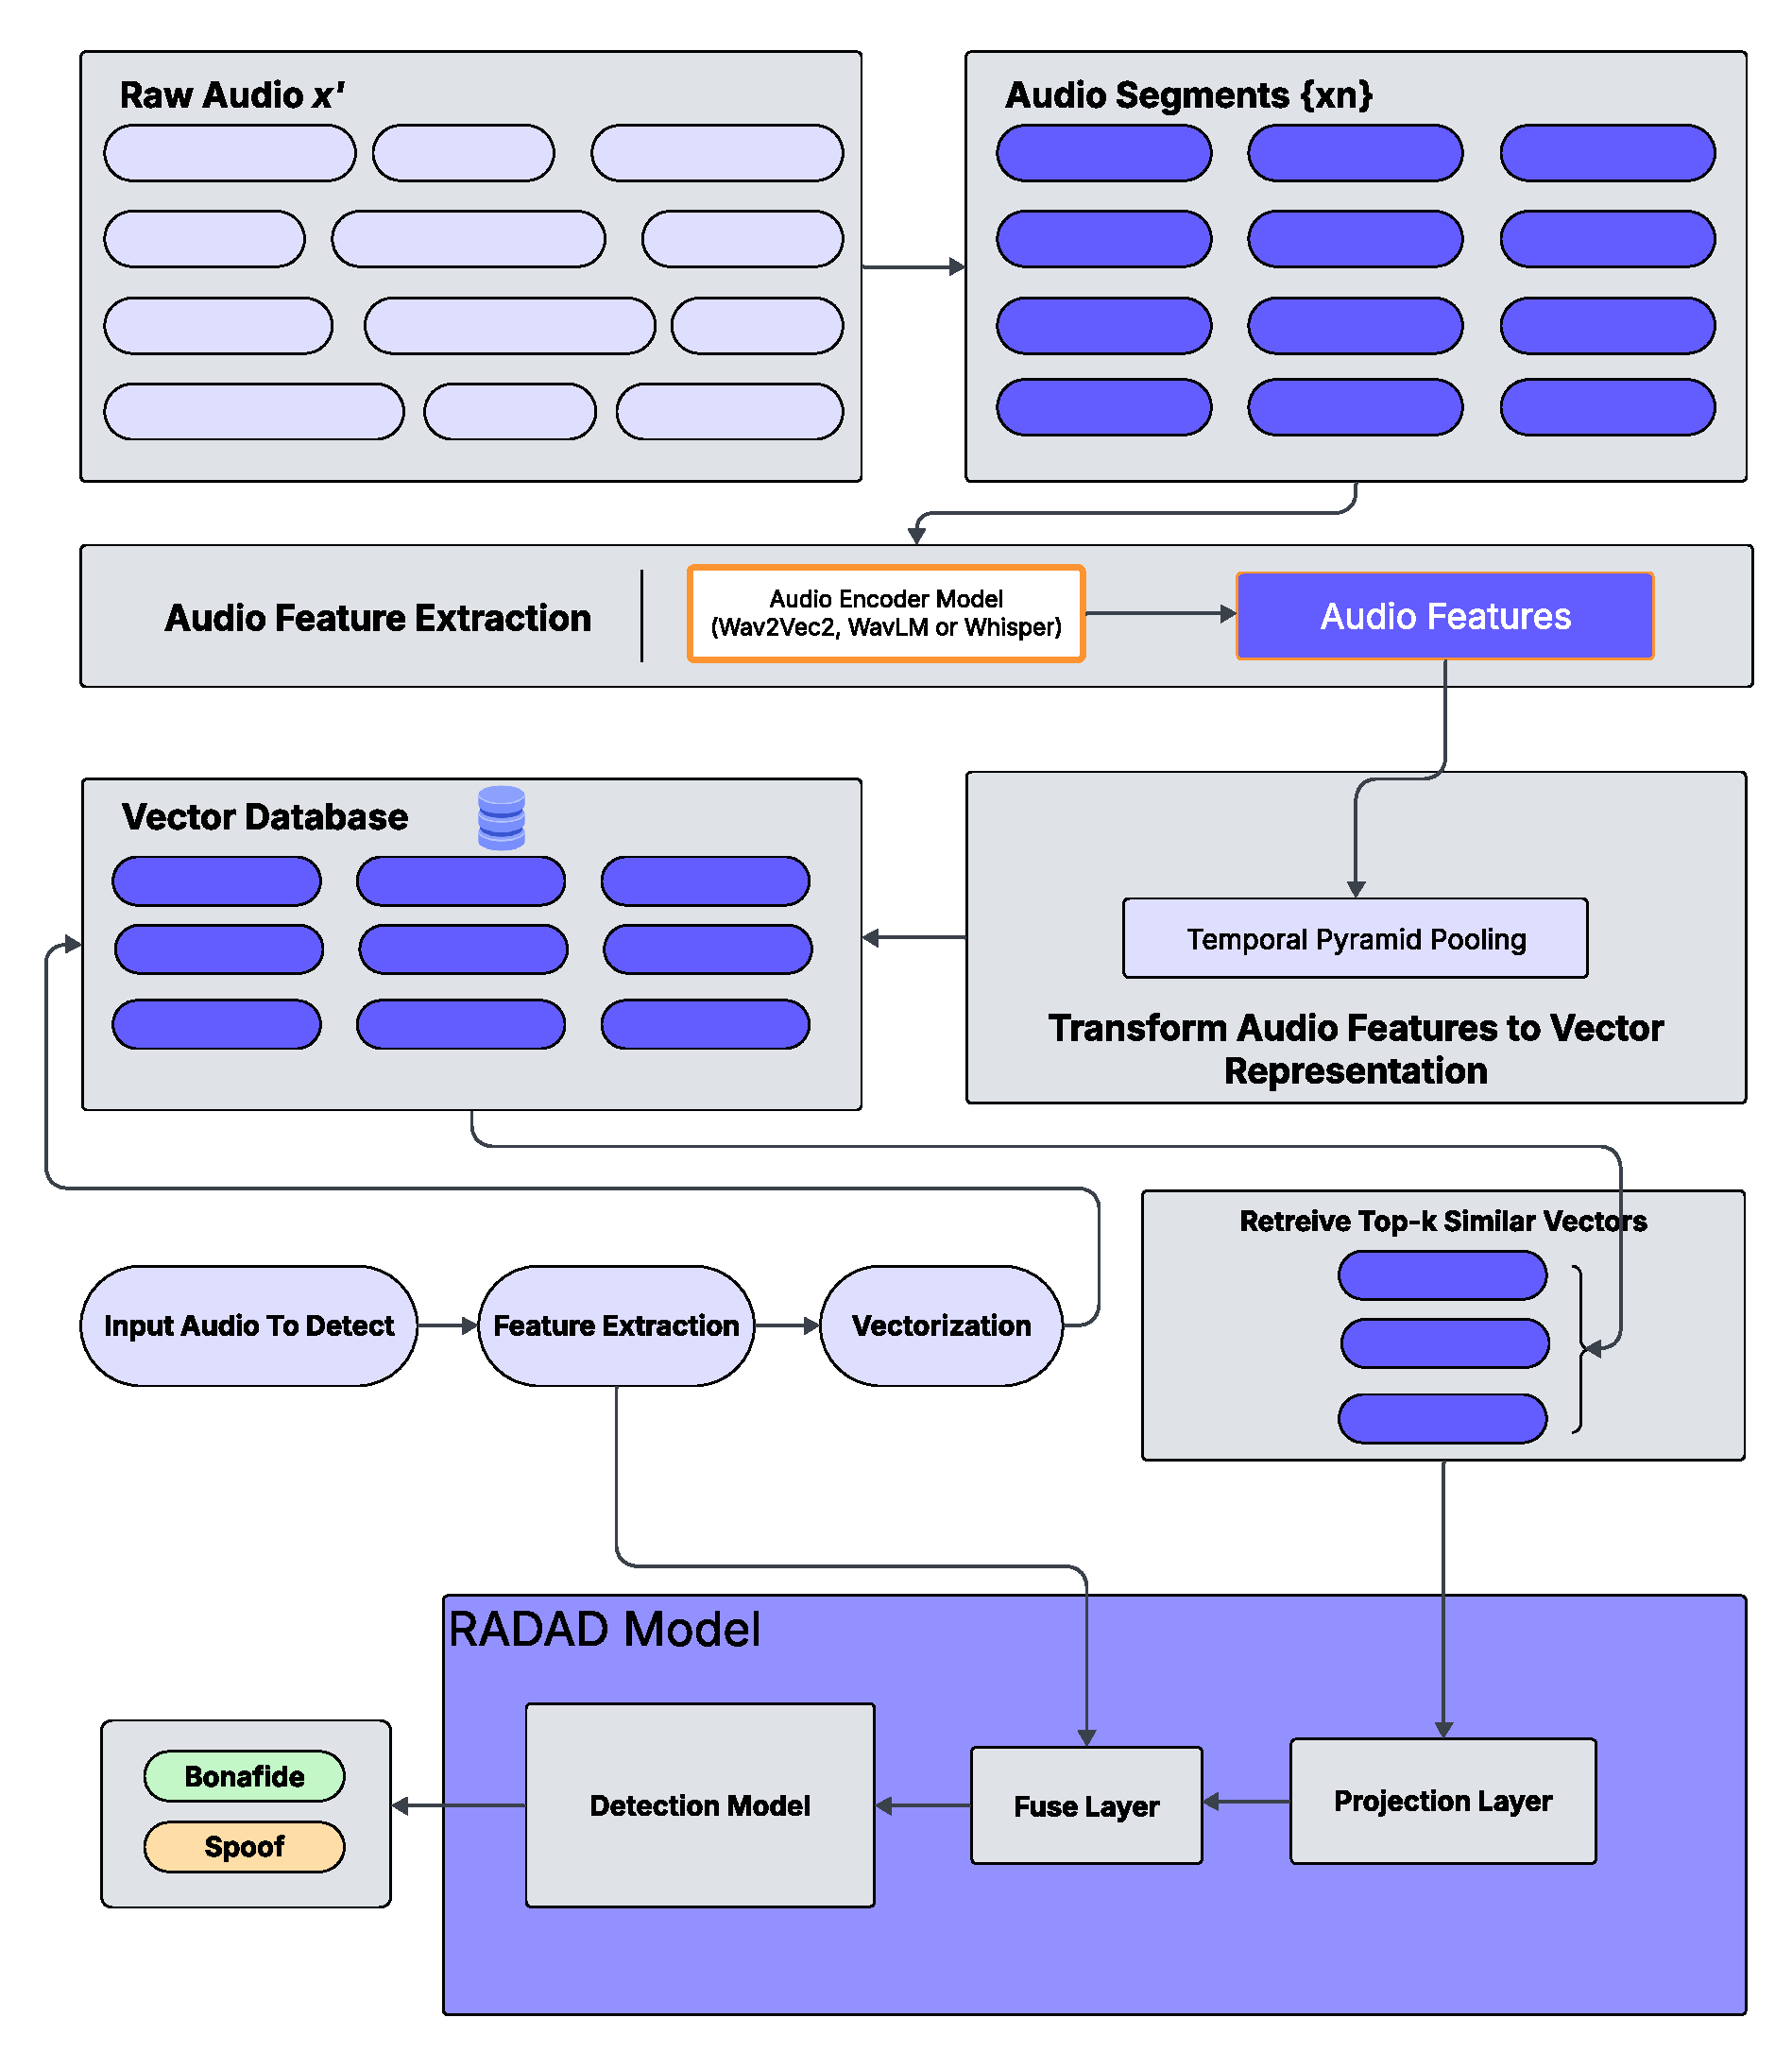
\includegraphics[width=0.7\textwidth]{figures/architecture.png}
%   \caption{Methodology.}
%   \label{fig:proj-arch}
% \end{figure}

% \subsection{Audio Vector Database Creation}\label{sec:methodology:step1}
% The foundation of our approach is a comprehensive vector database of speech representations of bonafide and synthetic samples. This database is constructed through a systematic process:

% \subsubsection{Audio Segmentation}\label{sec:methodology:step1:seg} 
% Raw audio recordings from verified sources are first divided into consistent temporal segments (typically 2-3 seconds), preserving acoustic continuity while enabling fine-grained analysis.
% \subsubsection{Feature Extraction}\label{sec:methodology:step1:feature} These segments undergo feature extraction using pre-trained self-supervised audio encoders-specifically, Wav2Vec2.0 \cite{baevski2020wav2vec}, WavLM \cite{Chen_2022}, or Whisper \cite{radford2023robust}. These models, having been trained on diverse speech corpora, capture rich spectro-temporal patterns characteristic of human speech.
% \subsubsection{Temporal Pyramid Pooling}\label{sec:methodology:step1:tpp} 
% To address variable-length inputs and reduce dimensionality, we implement Temporal Pyramid Pooling that transforms encoder-generated features into fixed-dimension vectors while preserving temporal dynamics critical for speech authenticity assessment.
% \subsubsection{Vector Storage}\label{sec:methodology:step1:vector} 
% The resulting embeddings are indexed in a vector database optimized for similarity search operations, with metadata linking each vector to its source audio characteristics.

% \subsection{Deepfake Detection Pipeline}\label{sec:methodology:pipe}
% When presented with an audio sample for authenticity verification, our system employs a retrieval-augmented classification approach:
% \subsubsection{Audio Encoding}\label{sec:methodology:step1:encoding} 
% The query audio undergoes identical processing as database entries-segmentation, feature extraction via the same encoder architecture, and vectorization through temporal pyramid pooling-ensuring representation consistency.

% \subsubsection{Similarity-Based Retrieval}\label{sec:methodology:step1:similarity} 
% We perform efficient similarity search within the vector database to identify the top-k most similar speech samples to the query. This similarity analysis reveals subtle discrepancies between authentic and synthetic speech patterns.

% \subsubsection{Contextual Projection}\label{sec:methodology:step1:projection} Retrieved vectors undergo transformation through a projection layer that creates a condensed latent representation of similar authentic references, capturing essential characteristics of genuine speech relevant to the query.

% \subsubsection{Augmented Classification}\label{sec:methodology:step1:classification}
% Finally, both the query representation and the projected reference context are fed into a lightweight detection model. This model leverages the contextual comparison to determine whether the input sample exhibits synthetic artifacts inconsistent with authentic speech patterns, classifying it as either bonafide or spoofed.

% By grounding detection decisions in reference to known authentic and synthetic samples rather than solely relying on learned classification boundaries, our approach maintains robustness against unfamiliar synthesis techniques. Moreover, the vector database can be continuously updated to incorporate emerging voice patterns, enabling adaptive defense against evolving deepfake technologies.


% The lightweight nature of the detection model, coupled with efficient vector search algorithms, enables practical deployment on resource-constrained devices while maintaining competitive accuracy with more computationally intensive end-to-end approaches.

\section{Methodology}\label{sec:methodology}

Traditional deepfake audio detectors learn a static, parametric boundary from training data: a front‑end encoder produces embeddings that a back‑end classifier maps to a binary decision. Although effective on in‑domain benchmarks, such systems degrade under distribution shift novel spoofing methods, unseen channel conditions, or new speakers because knowledge is frozen in weights that cannot adapt post‑deployment. Moreover, they score each utterance in isolation, discarding contextual cues (e.g., speaker identity or previously observed exemplars) that could regularize decisions. Their reliance on large transformers or ensembles also raises latency and energy costs, complicating real‑time or edge deployment.

This research work addresses these limitations with a retrieval‑augmented detector (RADAD). Instead of relying solely on a global decision boundary, RADAD grounds each prediction in a neighborhood of authenticated references retrieved from a vector database. This hybrid parametric–non‑parametric design provides instance‑level calibration: as acoustic or attack distributions evolve, the retrieved context adapts immediately, while the memory itself is incrementally updatable without retraining. As illustrated in Fig.~\ref{fig:methodology_comparison}, the conventional pipeline processes each sample independently through a front‑end encoder and back‑end classifier, whereas our architecture fuses the query representation with retrieved neighbors before final detection. The result is improved generalization, better calibration of scores, and a practical path to low‑latency deployment, since the external memory offloads modeling burden from the classifier and enables rapid, data driven adaptation.

\begin{figure}[h]
    \centering
    \begin{minipage}{0.45\textwidth}
        \centering
        
\includegraphics[width=\textwidth]{high_level_design_traditional_systems.pdf}
        \subcaption{Traditional Detection Pipeline}
        \label{fig:traditional}
    \end{minipage}
    \hfill
    \begin{minipage}{0.45\textwidth}
        \centering
        
\includegraphics[width=\textwidth]{high_level_design_proposed_method.pdf}
        \subcaption{Proposed Retrieval-Augmented Framework}
        \label{fig:proposed}
    \end{minipage}
    \caption{Comparison of traditional deepfake audio detection systems and the proposed retrieval-augmented approach. Traditional systems rely on fixed parametric classifiers, while the proposed method augments detection with dynamically retrieved contextual evidence from a vector database.}
    \label{fig:methodology_comparison}
\end{figure}

\subsection{Speaker Characteristics as Discriminative Evidence: Embedding Space Analysis}

The motivational foundation for retrieval-augmented detection rests on an empirical observation: bonafide and spoofed audio samples occupy distinctly separable regions of the learned embedding space, with separation arising from speaker specific acoustic characteristics. Self‑supervised models like WavLM, trained with speaker awareness, learn representations where bonafide utterances from the same speaker cluster coherently, while synthesis artifacts systematically displace spoofed samples from these natural speaker neighborhoods.

Fig.~\ref{fig:embedding_space} visualizes this geometric organization through Uniform Manifold Approximation and Projection (UMAP) of WavLM embeddings for bonafide and spoofed samples from the RITW dataset. The bonafide embedding space (left panel) exhibits tight speaker specific clustering: utterances from the same speaker remain spatially proximate, reflecting preservation of speaker identity and natural acoustic properties (prosodic contours, spectral consistency, voice quality). In contrast, the spoof embedding space (right panel) reveals fragmented, dispersed distributions: synthetic utterances targeting a specific speaker occupy anomalous positions adjacent to, but distinctly separated from, authenticated speaker clusters. This dispersion reflects systematic synthesis induced deviations rigid prosody, vocoder artifacts, unnatural micro-prosody that disrupt natural speaker coherence.

\begin{figure}[h]
    \centering
    \begin{minipage}{0.48\textwidth}
        \centering
        
\includegraphics[width=\textwidth]{umap_InTheWild_WAVLM_bonafide_top5x20.pdf}
        \subcaption{Bonafide Embeddings}
        \label{fig:umap_bonafide}
    \end{minipage}
    \hfill
    \begin{minipage}{0.48\textwidth}
        \centering
        
\includegraphics[width=\textwidth]{umap_InTheWild_WAVLM_spoof_top5x20.pdf}
        \subcaption{Spoof Embeddings}
        \label{fig:umap_spoof}
    \end{minipage}
    \caption{UMAP projections of WavLM embeddings (top-5 retrieval neighbors with multiplicity 20) for bonafide and spoofed utterances from the RITW dataset. Bonafide samples form speaker-coherent neighborhoods reflecting natural acoustic characteristics. Spoofed samples exhibit structured anomalies displaced from authentic clusters, providing geometric evidence for retrieval-based discrimination.}
    \label{fig:embedding_space}
\end{figure}

This embedding geometry motivates our retrieval mechanism: bonafide test queries retrieve neighbors from their speaker clusters (providing in-cluster counterfactual evidence), while spoofed queries retrieve neighbors exhibiting synthesis induced anomalies (providing out-of-cluster evidence). Critically, this discrimination occurs automatically without explicit speaker labels the learned representation space itself encodes speaker identity and authenticity. Temporal pyramid pooling amplifies this effect by preserving multi-scale speaker characteristics: coarse pooling captures long-term prosodic patterns endemic to individual speakers, while fine-grained pooling reveals frame-level synthesis artifacts.

\subsection{Retrieval-Augmented Framework: System Architecture}

This work proposes a retrieval-augmented framework for deepfake audio detection that conditions each decision on a neighborhood of authenticated speech, rather than relying solely on a global, parametric decision boundary. The framework comprises two stages, depicted in detail in Fig.~\ref{fig:radad_architecture}: (i) an offline pipeline that builds a vector database of temporally pooled embeddings for bona-fide and spoofed utterances; and (ii) an online detection pipeline that encodes a query, retrieves its most similar neighbors, and performs context-conditioned classification. The architectural design combines self-supervised feature extraction with temporal aggregation and retrieval based contextual fusion, enabling the system to leverage speaker specific evidence for robust deepfake detection.

\begin{figure}[!htb]
    \centering
    
\includegraphics[width=0.85\textwidth]{architecture.pdf}
    \caption{Architecture of the proposed retrieval-augmented framework for deepfake audio detection (RADAD). The offline phase constructs a vector database from training samples through feature extraction and temporal pyramid pooling. During inference, a query utterance is encoded, converted to a fixed-dimensional vector representation through TPP, and its nearest neighbors are retrieved from the database. A projection layer processes retrieved neighbors into a context vector through attention-based weighting, which is then fused with the query representation. A lightweight detection head processes the fused representation to produce the final spoof/bonafide classification.}
    \label{fig:radad_architecture}
\end{figure}

\subsubsection{Audio Vector Database Creation}

Let \(x \in \mathbb{R}^T\) denote a waveform sampled at \(f_s\). We first segment \(x\) into overlapping windows of length \(L\) (seconds) and hop \(H\):

\begin{equation}
x^{(m)} = \{x_{(m-1)H+1}, \ldots, x_{(m-1)H+L}\}, \quad M \approx \left\lceil \frac{T - L}{H} \right\rceil + 1
\end{equation}

This preserves local stationarity and yields a set \(\{x^{(m)}\}_{m=1}^{M}\) suitable for fine-grained analysis.

\paragraph{Self-supervised feature extraction} Each segment is mapped to a frame-level representation using a pre-trained, self-supervised encoder \(f_\theta\) drawn from Wav2Vec 2.0, WavLM, or the Whisper encoder:

\begin{equation}
\mathcal{H}^{(m)} = f_\theta(x^{(m)}) \in \mathbb{R}^{U_m \times D}
\end{equation}

where \(U_m\) is the number of encoder frames for segment \(m\) and \(D\) is the embedding dimension. These models trained on large, heterogeneous corpora capture rich spectro-temporal regularities that are known to benefit downstream detection tasks. Models like WavLM incorporate speaker-aware pre-training objectives, creating the speaker-coherent clustering observed in Fig.~\ref{fig:embedding_space}.

\paragraph{Temporal pyramid pooling (TPP)} To convert variable-length frame sequences into fixed dimensional descriptors while retaining multi-scale dynamics, we adopt temporal pyramid pooling. Let the time axis of \(\mathcal{H}^{(m)}\) be partitioned at level \(\ell\) into \(2^\ell\) equal bins \(\mathcal{P}_\ell = \{b_1, \ldots, b_{2^\ell}\}\). For an aggregation operator \(g\) (e.g., mean or mean+std), we define level-wise pooled summaries:

\begin{equation}
v^{(m)}_\ell = \left\{ g\left(\mathcal{H}^{(m)}_b\right) \mid b \in \mathcal{P}_\ell \right\} \in \mathbb{R}^{2^\ell \times D}
\end{equation}

Concatenating across levels and averaging over segments yields the utterance-level embedding:

\begin{equation}
q = \frac{1}{M} \sum_{m=1}^{M} \text{concat}\left(v^{(m)}_0, \ldots, v^{(m)}_{L_{\text{pyr}}-1}\right) \in \mathbb{R}^d, \quad d = D \sum_{\ell=0}^{L_{\text{pyr}}-1} 2^\ell
\end{equation}

TPP preserves coarse-to-fine temporal cues that are often perturbed by synthesis (e.g., prosody, micro-pauses), enabling the embedding space to reflect both speaker-level characteristics and frame-level anomalies as shown in Fig.~\ref{fig:embedding_space}.

\paragraph{Vector storage and indexing} We store triplets \((q_i, y_i, \mathcal{M}_i)\) for each utterance \(i\), where \(y_i \in \{0, 1\}\) indicates spoof/bona-fide and \(\mathcal{M}_i\) contains metadata (e.g., speaker). For efficient similarity search, we L2-normalize embeddings, \(\tilde{q} = q / \|q\|_2\), so inner product equals cosine similarity. We use FAISS to build an index (e.g., flat IP, IVF-PQ, or HNSW), enabling sub-linear k-NN queries in large memories, while preserving the speaker-coherent clustering shown in Fig.~\ref{fig:embedding_space}.

\subsubsection{Deepfake Detection Pipeline}

At inference time, the query utterance undergoes the same pipeline (Segmentation, Encoder, TPP) to produce \(q \in \mathbb{R}^d\). We then retrieve its \(k\) nearest neighbors by cosine similarity:

\begin{equation}
\mathcal{N}(q) = \{q_{i_1}, \ldots, q_{i_k}\}, \quad i_j \in \arg\max_i \tilde{q}^\top \tilde{q}_i
\end{equation}

To avoid trivial self-matches, the exact query file is excluded when the database originates from the same split. Over-retrieval (e.g., \(k+10\)) is used in practice to retain \(k\) neighbors after self-exclusion. As illustrated in Fig.~\ref{fig:radad_architecture}, the retrieved neighbors are projected and fused with the query representation before being passed to the detection head.

\paragraph{Contextual projection} The retrieved set is summarized through a learnable projection \(h_\phi : \mathbb{R}^d \to \mathbb{R}^{d'}\) and similarity-based attention:

\begin{equation}
c = \sum_{j=1}^{k} \alpha_j h_\phi(q_{i_j}), \quad \alpha_j = \frac{\exp(\tau s_j)}{\sum_{\ell=1}^{k} \exp(\tau s_\ell)}
\end{equation}

where \(s_j = \tilde{q}^\top \tilde{q}_{i_j}\) and \(\tau > 0\) is a temperature that controls neighbor sharpness. This yields a compact context vector \(c \in \mathbb{R}^{d'}\) that reflects the empirical manifold around the query, with attention-weighted aggregation ensuring that neighbors closer in speaker and authenticity space contribute more strongly.

\paragraph{Fusion and detection} We fuse the query and its context via a linear map \(W_f \in \mathbb{R}^{d'' \times (d+d')}\):

\begin{equation}
z = W_f [q; c] \in \mathbb{R}^{d''}
\end{equation}

A lightweight classifier \(g_\psi\) (two to three fully connected layers with normalization and non-linearity) outputs a logit \(\ell \in \mathbb{R}\) and posterior \(\hat{p} = \sigma(\ell)\) for the bona-fide class:

\begin{equation}
\ell = g_\psi(z), \quad \hat{p} = \sigma(\ell) = \frac{1}{1 + \exp(-\ell)}
\end{equation}

\paragraph{Training objective and regularization} Given labeled utterances \(\{(q_i, y_i)\}_{i=1}^{N}\), we minimize a class-weighted logistic loss to handle label skew:

\begin{equation}
\mathcal{L}(\theta, \phi, \psi) = -\frac{1}{N} \sum_{i=1}^{N} \left[ \lambda_{y_i} \log \hat{p}_i + (1-y_i) \log(1-\hat{p}_i) \right]
\end{equation}

where \(\lambda > 0\) up-weights the bona-fide class when needed. Gradients flow through \(h_\phi\) and \(g_\psi\) (and optionally \(f_\theta\) if fine-tuned). Retrieval is treated as a fixed operator conditioned on the current \(q\). This work additionally employ weight decay and gradient clipping to stabilize optimization early in training when the memory is still sparse.

\paragraph{Complexity and deployment} The parametric inference cost for the MLP-based detection is \(\mathcal{O}(d'' H)\) for an MLP width \(H\). The non-parametric cost is dominated by k-NN search; with FAISS and product quantization or HNSW, retrieval scales sub-linearly with database size and supports low-latency operation. Notably, the external memory is updatable: emergent spoofing styles can be incorporated by appending new embeddings without retraining \(g_\psi\).

\paragraph{Rationale} By anchoring a decision in a neighborhood of authenticated speech, the detector inherits non-parametric robustness: as the distribution drifts, \(\mathcal{N}(q)\) adapts, providing instance-level calibration of the score. The speaker-aware organization of the embedding space (Fig.~\ref{fig:embedding_space}) ensures that retrieved neighbors naturally reflect speaker-specific acoustic profiles and authenticity patterns. This complements strong self-supervised encoders that furnish stable, speaker-aware features, while TPP preserves multi-scale temporal cues that are perturbed in synthetic speech. In aggregate, the retrieval-augmented approach implements a compact, memory-centric alternative to purely parametric detectors, yielding improved generalization to unseen manipulation techniques while maintaining computational efficiency suitable for edge deployment.
% -----------------------------
% Bibliography placeholders
% -----------------------------
% Add these works to your .bib:
% \bibitem{jung2022aasist} J.-W. Jung et al., ``AASIST: Audio Anti-Spoofing using Integrated Spectro-Temporal Graph Attention Networks,'' 2022.
% \bibitem{tak2021end} H. Tak et al., ``End-to-End Anti-Spoofing with RawNet2,'' 2021.
% \bibitem{alzantot2019lcnn} M. Alzantot et al., ``Deep Residual LCNN for Spoofing Detection,'' 2019.
% \bibitem{muller2022rawgatst} N. Müller et al., ``Does Audio Deepfake Detection Generalize? RawGAT-ST,'' 2022.
% \bibitem{baevski2020wav2vec} A. Baevski et al., ``wav2vec 2.0: A Framework for Self-Supervised Learning of Speech Representations,'' 2020.
% \bibitem{Chen_2022} S. Chen et al., ``WavLM: Large-Scale Self-Supervised Pre-Training for Full Stack Speech Processing,'' 2022.
% \bibitem{radford2023robust} A. Radford et al., ``Robust Speech Recognition via Large-Scale Weak Supervision,'' 2023.
% \bibitem{He_2014} K. He et al., ``Spatial Pyramid Pooling in Deep Convolutional Networks,'' 2014.
% \bibitem{he2019stnet} D. He et al., ``StNet: Local and Global Spatial-Temporal Modeling for Action Recognition,'' 2019.
% \bibitem{johnson2019billion} J. Johnson et al., ``Billion-Scale Similarity Search with GPUs,'' 2019.
% \bibitem{jegou2010product} H. Jégou et al., ``Product Quantization for Nearest Neighbor Search,'' 2010.
% \bibitem{malkov2018efficient} Y. Malkov and D. Yashunin, ``Efficient and Robust Approximate Nearest Neighbor Search Using HNSW,'' 2018.
% \bibitem{khandelwal2019generalization} U. Khandelwal et al., ``Generalization through Memorization: Nearest Neighbor Language Models,'' 2019.
% \bibitem{lewis2020retrieval} P. Lewis et al., ``Retrieval-Augmented Generation for Knowledge-Intensive NLP,'' 2020.


% % ==============================
% % References to add (BibTeX keys suggested)
% % ==============================

% % baevski2020wav2vec
% % chen2022wavlm
% % radford2023whisper
% % he2015spp
% % zha2015tpp
% % johnson2019faiss
% % khandelwal2020knnlm
% % lewis2020rag
% % jegou2011pq
% % malkov2018hnsw


\section{Experimental Setup}\label{sec:Experiments}

This section details the experimental design, implementation, and evaluation protocol for the proposed Retrieval-Augmented framework for Deepfake Audio Detection (RADAD). Experiments were conducted with three front-end feature extractors Wav2Vec 2.0, Whisper, and WavLM plugged into a shared downstream architecture and training loop so that differences in performance can be attributed primarily to the representation quality rather than confounding implementation details.

\subsection{Datasets and Metrics}\label{sec:datasets-metrics}

\subsubsection{Release In The Wild (RITW)}
The proposed method is evaluated on the \emph{In‑the‑Wild Audio Deepfake} \cite{müller2024doesaudiodeepfakedetection} corpus (the release\_in\_the\_wild subset), a collection of short speech clips sourced from publicly available media featuring English‑speaking celebrities and public figures. The corpus contains both bona‑fide recordings and manipulated speech (text‑to‑speech and voice conversion) for overlapping speakers, thus inducing challenging, naturally diverse channel and content conditions (broadcast interviews, talks, podcasts, and web audio). Following the dataset description, it comprises recordings from \textbf{58 speakers}, with approximately \textbf{20.8 hours} of bona‑fide speech and \textbf{17.2 hours} of spoofed speech, providing broad coverage across subjects and content types (we standardize all audio to 16\,kHz for compatibility with the feature extractors). For our experiments, we construct an \textbf{80/20 split} that is stratified by label to preserve the bona‑fide/spoof ratio across folds. We treat bona‑fide as the positive class ($y{=}1$) and spoof as the negative class ($y{=}0$). Table~\ref{tab:data_splits} summarizes the final split statistics used in our runs.


\begin{table}[!htb]
\centering
\small
\caption{Dataset Composition and Class Balance}
\label{tab:data_splits}
\begin{tabular}{l l r r r}
\toprule
\textbf{Dataset} & \textbf{Split} & \textbf{Total} & \textbf{Bona-fide \# (\%)} & \textbf{Spoof \# (\%)} \\
\midrule
In-The-Wild & Train & 25{,}423 & 9{,}453 (37.18\%) & 15{,}970 (62.82\%) \\
In-The-Wild & Val   &  6{,}356 & 2{,}363 (37.18\%) &  3{,}993 (62.82\%) \\
\midrule
FakeAVCeleb & Train & 17{,}252 & 9{,}085 (52.66\%) &  8{,}167 (47.34\%) \\
FakeAVCeleb & Val   &  4{,}314 & 2{,}272 (52.67\%) &  2{,}042 (47.33\%) \\
\bottomrule
\end{tabular}
\end{table}

\subsubsection{FakeAVCeleb}
We also evaluate on \emph{FakeAVCeleb}, a multimodal in‑the‑wild benchmark containing bona‑fide and manipulated utterances for celebrity identities, curated from publicly available media~\cite{khalid2021fakeavceleb}. Similar to RITW, the audio exhibits heterogeneous channel characteristics and content styles, but the class balance is closer to even, making it complementary for robustness analysis. We resample all audio to 16\,kHz and follow the same preprocessing pipeline (segmentation and temporal pooling) to keep the representation space comparable across datasets. We adopt an \textbf{80/20 stratified split} by label; the resulting statistics are shown in Table~\ref{tab:data_splits}.

\subsubsection{Detection Evaluation Metrics}
We report standard detection metrics per epoch on the validation split: \textbf{Accuracy}, \textbf{ROC AUC}, and error‑rate measures. Let $s(x)\in\mathbb{R}$ denote the detector score (we use raw logits), with larger values indicating stronger evidence for bona‑fide. For a threshold $\tau$, the \emph{false positive rate} (accepting spoof as bona‑fide) and \emph{false negative rate} (rejecting bona‑fide) are

\[
\mathrm{FPR}(\tau) \;=\; \mathbb{P}\big(s(x)\ge \tau \,\big|\, y{=}0\big), 
\qquad
\mathrm{FNR}(\tau) \;=\; \mathbb{P}\big(s(x)< \tau \,\big|\, y{=}1\big).
\]

The \textbf{Equal Error Rate (EER)} is computed by scanning unique thresholds and finding $\tau^\star$ where $\mathrm{FPR}(\tau^\star)\approx \mathrm{FNR}(\tau^\star)$; we report $\mathrm{EER}=\mathrm{FPR}(\tau^\star)$ as a percentage. 

In addition, we track operating‑point classification metrics derived from the confusion matrix: \textbf{True Positive Rate (TPR/Recall)} $=\frac{\mathrm{TP}}{\mathrm{TP}+\mathrm{FN}}$, \textbf{True Negative Rate (TNR/Specificity)} $=\frac{\mathrm{TN}}{\mathrm{TN}+\mathrm{FP}}$, \textbf{Precision} $=\frac{\mathrm{TP}}{\mathrm{TP}+\mathrm{FP}}$, and the \textbf{F1‑score}

\[
\mathrm{F1} \;=\; \frac{2\,\mathrm{Precision}\cdot \mathrm{Recall}}{\mathrm{Precision}+\mathrm{Recall}}.
\]

AUC is computed as the area under the ROC curve via trapezoidal integration, and Accuracy is the fraction of correctly classified clips at the chosen threshold. Unless stated otherwise, bona‑fide is the positive class.

\subsubsection{Retrieval Quality Metrics}
Beyond detection accuracy, we assess the relevance and quality of retrieved neighbors through speaker-based and content-based metrics. These metrics evaluate whether the retrieval mechanism produces meaningful neighborhoods that align with speaker identity and utterance content. We employ the following complementary measures:

\textbf{Speaker-Based Metrics:} Given a query utterance with associated speaker identity, we analyze the $k$ nearest retrieved neighbors. Let $\mathcal{R}(q) = \{r_1, r_2, \ldots, r_k\}$ denote the retrieved neighbors ordered by similarity, with speaker labels $s(r_i)$ for neighbor $r_i$. We define:

\begin{equation}
\mathrm{Top\text{-}1\,Acc@k} \;=\; \frac{1}{N_q} \sum_{q=1}^{N_q} \mathbb{1}\{s(r_1) = s(q)\},
\end{equation}

measuring the proportion of queries where the most similar retrieved sample matches the query speaker. This metric directly assesses speaker-aware organization of the embedding space.

\begin{equation}
\mathrm{Speaker\,Precision@k} \;=\; \frac{1}{N_q} \sum_{q=1}^{N_q} \frac{|\{i \in [1,k] : s(r_i) = s(q)\}|}{k},
\end{equation}

computing the average fraction of retrieved neighbors originating from the same speaker as the query, quantifying how well the retriever clusters same-speaker utterances within the top-k neighborhood.

\begin{equation}
\mathrm{Speaker\,Recall@k} \;=\; \frac{1}{N_q} \sum_{q=1}^{N_q} \frac{|\{i \in [1,k] : s(r_i) = s(q)\}|}{|\{j : s(x_j) = s(q)\}|},
\end{equation}

measuring the fraction of same-speaker samples in the database retrieved in the top-k results, assessing coverage of speaker-relevant exemplars.

\begin{equation}
\mathrm{Speaker\,MRR} \;=\; \frac{1}{N_q} \sum_{q=1}^{N_q} \frac{1}{\min\{i : s(r_i) = s(q)\}},
\end{equation}

where MRR denotes Mean Reciprocal Rank, measuring the average rank of the first same-speaker neighbor. This metric rewards retrieval systems that place speaker-matching samples early in the ranking.

\textbf{Content-Based Metrics:} To assess whether retrieved neighbors represent relevant content, we apply content-based similarity through transcription. Let $c(x)$ denote the content representation (word-level transcription) of utterance $x$. We compute:

\begin{equation}
\mathrm{Content\,Jaccard@k} \;=\; \frac{1}{N_q} \sum_{q=1}^{N_q} \frac{|\{w \in c(q)\} \cap |\{w \in c(r_i)\}|}{|\{w \in c(q)\} \cup |\{w \in c(r_i)\}|},
\end{equation}

measuring Jaccard similarity (intersection over union of word tokens) between query content and retrieved neighbors, quantifying lexical overlap and content consistency.

\begin{equation}
\mathrm{Content\,F1@k} \;=\; \frac{1}{N_q} \sum_{q=1}^{N_q} \frac{2 \cdot P_{\text{content}} \cdot R_{\text{content}}}{P_{\text{content}} + R_{\text{content}}},
\end{equation}

where $P_{\text{content}}$ (precision) measures the fraction of retrieved neighbor tokens present in query content, and $R_{\text{content}}$ (recall) measures the fraction of query tokens retrieved in neighbor content. F1-score balances precision and recall for a comprehensive content-similarity assessment.

These retrieval quality metrics serve two purposes: (i) they provide interpretability into retrieval mechanism behavior, revealing whether retrieved neighbors are speaker-consistent or content-consistent; and (ii) they enable comparative analysis across feature extractors to understand how representation design influences neighborhood structure. Metrics closer to 1.0 indicate more coherent and speaker-aligned retrieval, while lower values suggest potential retrieval instability or poor speaker-embedding organization.

\subsection{Implementation details}
This section presents the practical implementation of RADAD, detailing the core architectural components, training methodology, and experimental configuration. The system is realized through a modular design that combines neural feature extraction with efficient retrieval mechanisms, enabling end-to-end training while maintaining computational efficiency suitable for deployment. Implementation specifics include preprocessing parameters, vectorization strategies, and optimization procedures that collectively ensure reproducibility and performance consistency across experimental runs.

\subsubsection{Retrieval-Augmented Architecture}
The method integrates instance retrieval with discriminative classification. Each input utterance is segmented (via AudioSegmenter), embedded by the chosen feature extractor, and temporally pooled with TemporalPyramidPooling (TPP) to produce a fixed-dimensional query vector $q \in \mathbb{R}^{D_{\text{tpp}}}$. A FAISS-based VectorDatabase pre-built from the training split returns the top-K neighbors for each query. These neighbors are projected by an attention-style ProjectionLayer to produce a compact context vector $c \in \mathbb{R}^{D_{\text{proj}}}$. The query and context are fused by a learned linear map,

\begin{equation}\label{eq:fuse}
    z = W_f \left[ q \, \| \, c \right] + b_f \in \mathbb{R}^{D_{\text{proj}}}
\end{equation}

which is then consumed by a lightweight MLP (DetectionModel) to produce a logit $s \in \mathbb{R}$ where larger values indicate greater bona-fide likelihood. This ``query + context'' pattern is implemented end-to-end in the unified RADADModel class, encapsulating projection, fusion, and detection for a single checkpoint and optimizer state.

\subsubsection{Training Protocol}
Training uses mixed precision (torch.amp), gradient clipping, and Adam optimizers. To counter class imbalance, we compute a corpus-specific positive class weight and train with weighted BCE-with-logits:

\begin{equation}\label{eq:bce}
    \mathcal{L} = -\frac{1}{N}\sum_{i=1}^{N} \left[ w \, y_i \, \log\sigma(s_i) + (1-y_i) \, \log\left(1-\sigma(s_i)\right) \right]
\end{equation}

where $y_i \in \{0,1\}$, $s_i$ is the model logit, $\sigma(\cdot)$ is the sigmoid, and $w$ is the estimated $\text{pos\_weight} = \frac{\#\text{neg}+1}{\#\text{pos}+1}$.

We monitor batch-level diagnostics such as gradient norms and the fraction of non-zero retrieved neighbors (proxy for retrieval health). To avoid degenerate retrieval on validation, self-matches are excluded by filename.

The vector database is constructed once from training vectors using FAISS; at inference/training time, we over-retrieve $(K+10)$ to allow self-exclusion while still returning exactly $K$ neighbors after filtering. When retrieval yields fewer than $K$ results (e.g., very small databases), we pad with zero-vectors to maintain shape stability. All experiments are performed for 10 epochs on a single NVIDIA T4 GPU, and inference follows the same 16 kHz preprocessing.


% \section{Results}\label{sec:results}

% \begin{figure}[!htb]
%   \centering
%   \includegraphics[width=0.7\textwidth]{figures/ritw-radad-auc_curve.png}
%   \caption{AUC curve comparison.}
%   \label{fig:auc_curve}
% \end{figure}


% We evaluate the proposed Retrieval-Augmented Deepfake Audio Detector (RADAD) on the Release In The Wild evaluation split across three front-end encoders—Wav2Vec2, Whisper, and WavLM—while holding the retrieval and decision head constant. Unless noted otherwise, models are trained for 10 epochs on a single NVIDIA T4 and assessed after each epoch. Performance is reported in terms of accuracy and ROC AUC over the validation set, and we additionally compute (i) pooled Equal Error Rate (EER)—the operating point where the false acceptance rate equals the false rejection rate when treating the logits as bona-fide scores—and (ii) macro EER, obtained by averaging per-speaker EERs over speakers that contain both bona-fide and spoofed utterances.

% Fig. \ref{fig:auc_curve} provides the AUC trajectory per epoch for all three front-ends. WavLM achieves the highest AUC throughout training, exceeding 0.95 by epoch 2 and plateauing near 0.98 by the final epoch. Whisper follows closely, converging to $\approx$ 0.97, while Wav2Vec2 lags initially but improves steadily to $\approx$ 0.92 by epoch 10. The ordering mirrors the representational capacity of the respective encoders on in-the-wild speech with diverse channel conditions: WavLM’s large-scale masked prediction pretraining with integrated speaker/phonetic cues appears to yield embeddings that are better aligned with the retrieval objective, resulting in stronger separability between bona-fide and spoofed samples.

% \begin{figure*}[!htb]
%         \centering
%         \begin{subfigure}[b]{0.3\textwidth}  
%             \centering 
%             \includegraphics[width=\textwidth]{figures/ritw_wavlm_trainval-loss.png}
%             \caption[WavLM train/val loss.]%
%             {{\small WavLM}}    
%             \label{fig:wavLM}
%         \end{subfigure}
%         \hfill
%         \begin{subfigure}[b]{0.3\textwidth}   
%             \centering 
%             \includegraphics[width=\textwidth]{figures/ritw_wav2vec2_trainval-loss.png}
%             \caption[Wav2vec2 train/val loss.]%
%             {{\small Wav2vec2}}    
%             \label{fig:wav2vec2}
%         \end{subfigure}
%         \hfill
%         \begin{subfigure}[b]{0.3\textwidth}   
%             \centering 
%             \includegraphics[width=\textwidth]{figures/ritw_whisper_trainval-loss.png}
%             \caption[Whisper train/val loss.]%
%             {{\small Whisper}}    
%             \label{fig:whisper}
%         \end{subfigure}
%         \caption[ Train/val loss curves for RADAD model with different feature extractors. ]
%         {\small Train/val loss curves for RADAD model with different feature extractors.} 
%         \label{fig:loss_curves}
%     \end{figure*}

% Fig. \ref{fig:loss_curves} plot the train/validation loss curves for RADAD with Wav2Vec2, Whisper, and WavLM front-ends, respectively. All three settings exhibit stable convergence within ten epochs, with validation loss decreasing monotonically for WavLM and Whisper and showing mild non-monotonicity for Wav2Vec2 around epochs 6–8. Importantly, the gaps between training and validation curves remain small across the run, indicating limited overfitting even without early stopping. This behavior is consistent with the inductive bias introduced by the retrieval branch: nearest-neighbor contextualization regularizes the decision boundary by anchoring predictions to semantically similar real recordings, which in turn reduces variance in the learned classifier.

% \begin{table}[t]
% \centering
% \caption{Comparison with other anti-spoofing systems on the \textit{In The Wild} evaluation set, reported in terms of EER (\%).}
% \label{tab:inthewild_eer}
% \begin{tabular}{lcc}
% \toprule
% \textbf{System} & \textbf{EER (\%)} \\
% \midrule
% RawGAT-ST ~\cite{müller2024doesaudiodeepfakedetection} & 37.81 \\
% Wav2Vec, HuBERT, Conformer \& attention ~\cite{wang2023detection} & 36.84 \\
% XLS-R \& Res2Net ~\cite{yi2023audiodeepfakedetectionsurvey} & 36.62 \\
% MPE \& SENet ~\cite{wang2024multi} & 29.62 \\
% Spec \& POI-Forensics ~\cite{pianese2022deepfake} & 25.14 \\
% XLS-R, WavLM, HuBERT \& Fusion ~\cite{yang2024robust} & 24.27 \\
% XLS-R \& RawNet \& ASSIST ~\cite{tak2022automatic} & 10.46 \\
% XLS-R \& SLS ~\cite{zhang2024audio} & 7.46 \\
% \textbf{Ours (RADAD-WavLM)} & \textbf{5.41} \\
% \bottomrule
% \end{tabular}
% \end{table}


% Table \ref{tab:inthewild_eer} compares our best RADAD-WavLM configuration to prior anti-spoofing systems on the In-The-Wild evaluation set, using EER (\%) as the common metric. Our model obtains 5.41\% EER, surpassing recent strong baselines, including XLS-R \& SLS (7.46\%) and XLS-R + RawNet + ASSIST (10.46\%). Relative to prior best, RADAD-WavLM reduces EER by ~27.5\% absolute (7.46 → 5.41) and by 27.5\% / 7.46 $\approx $ 26.6\% relative. This gain is particularly notable given that RADAD uses a compact classification head and relies on retrieval to inject non-parametric context, rather than adding deeper parametric back-ends. In practice, the EER operating point $\tau^*$ is determined by scanning unique logit thresholds and selecting $\tau^* = argmin_\tau |FPR(\tau)-FNR(\tau)|;$ empirically $\tau^*$ aligned closely with the thresholds that maximize validation AUC, suggesting a well-calibrated score distribution.
\section{Results}\label{sec:results}

This section systematically presents the empirical findings of the proposed Retrieval Augmented Framework for Deepfake Audio Detection (RADAD) across two benchmark corpora: \emph{Release in the Wild} (RITW) and \emph{FakeAVCeleb}. The results are organized to highlight overall system performance on each dataset, provide direct comparative analysis against leading anti-spoofing methods, and assess the incremental contribution of retrieval augmentation relative to purely parametric baselines. Unless otherwise specified, all experiments employ a standardized training protocol of 10 epochs, with models evaluated at convergence. Core metrics including accuracy, area under the ROC curve (AUC), equal error rate (EER), and class-wise operating characteristics are reported to enable rigorous comparison. The supporting quantitative endpoints are presented sequentially in Tables~\ref{tab:ablation_metrics}–\ref{tab:fakeavceleb_acc}, with each table contextualizing the findings according to dataset and evaluation paradigm.



% \begin{figure}[!htb]
%   \centering
%   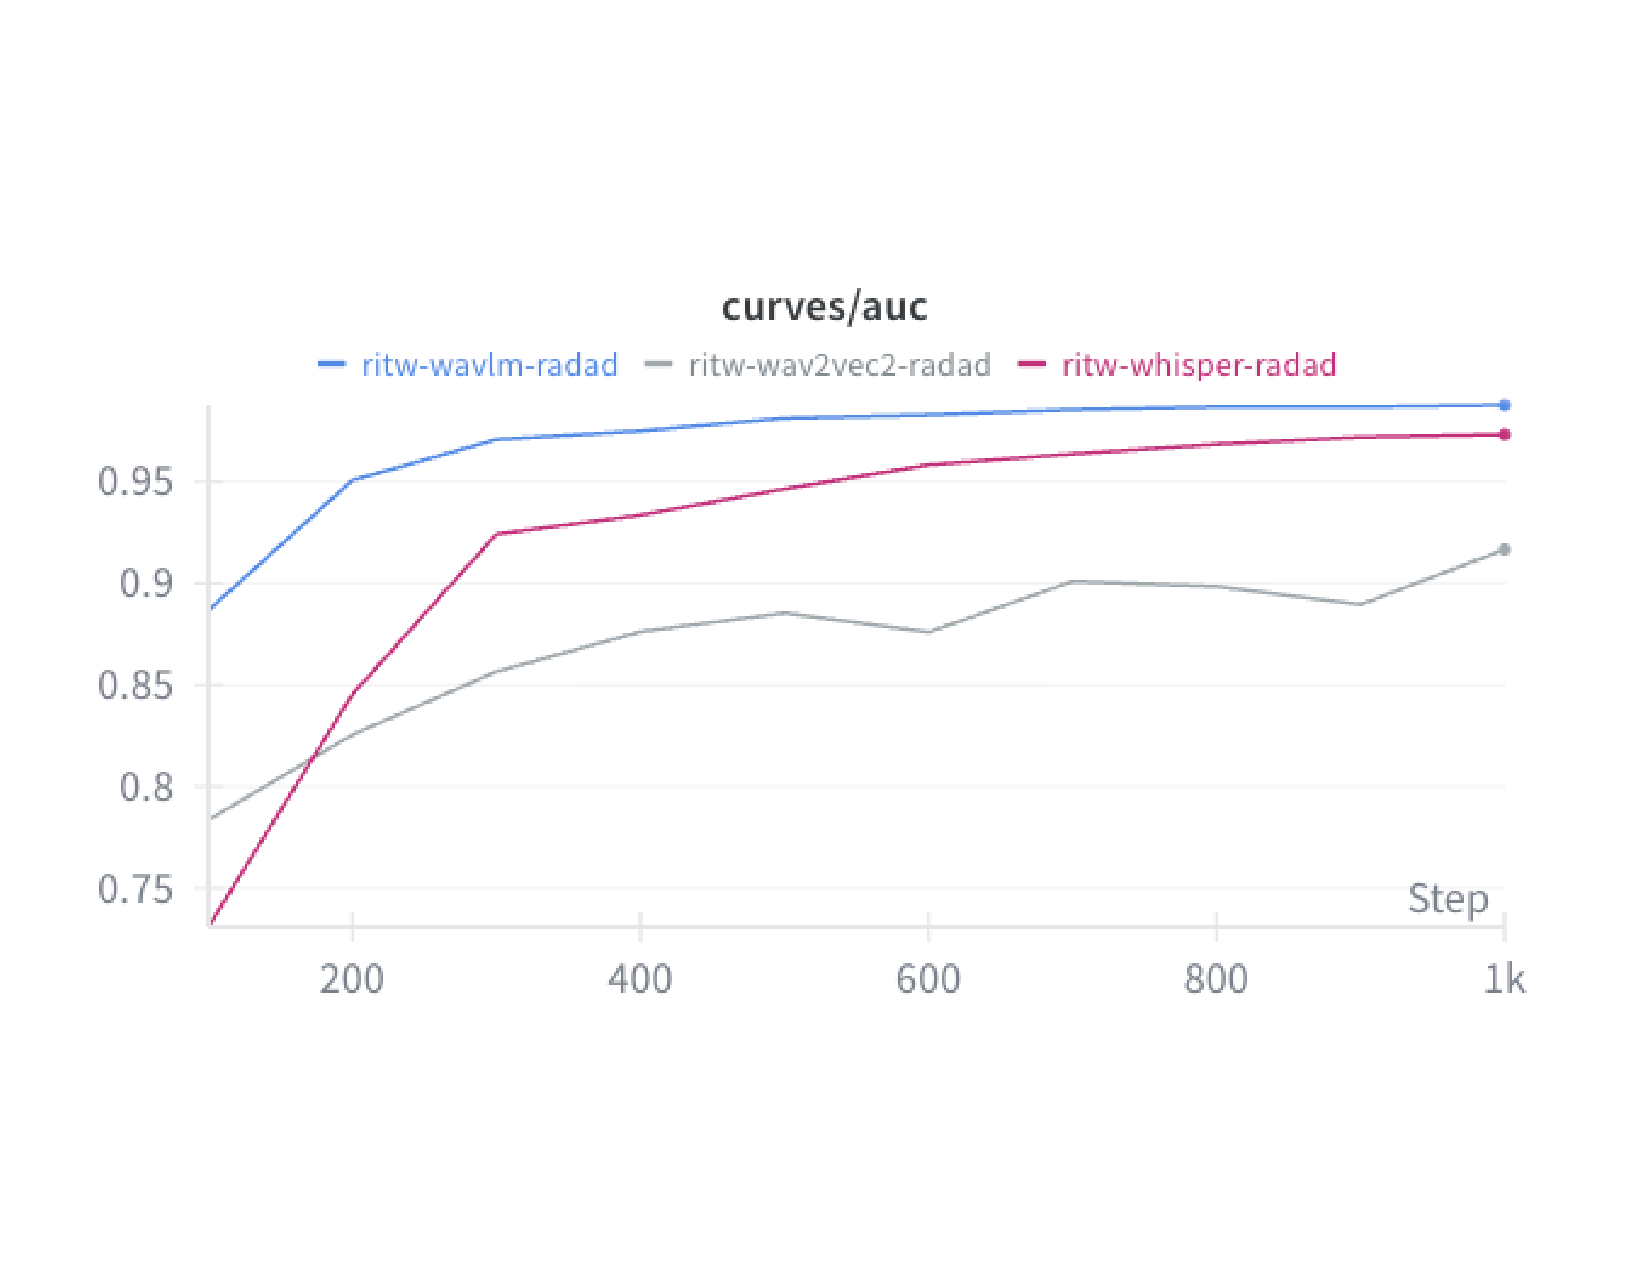
\includegraphics[width=0.7\textwidth]{figures/auc_curve.pdf}
%   \caption{ROC--AUC trajectory of RADAD over epochs on the \textit{Release In The Wild} validation split.}
%   \label{fig:auc_curve}
% \end{figure}



\subsection{Evaluation on \emph{Release in the Wild} Dataset}
\label{subsec:results-ritw}

In order to provide a rigorous comparative evaluation, we present two tables quantifying the performance of RADAD and relevant baselines on the \textit{Release in the Wild} (RITW) dataset. Notably, Table~\ref{tab:ablation_metrics} reports the results obtained by running our evaluation protocol and external baselines on the exact same dataset splits, while Table~\ref{tab:inthewild_eer} collates the equal error rate (EER) baselines as published in prior works.

\begin{table}[h]
\centering
\caption{Comparison of Key Metrics on \textit{Release In The Wild} Evaluation Set}
\label{tab:ablation_metrics}
\begin{tabular}{lccc}
\toprule
\textbf{System} & \textbf{Accuracy (\%)} & \textbf{AUC (\%)} & \textbf{EER (\%)} \\
\midrule
XLS-R \& SLS~\cite{zhang2024audio} & 88.25 & 97.72 & 7.28 \\
\textbf{Proposed (RADAD+WavLM)} & \textbf{90.22} & \textbf{98.83} & \textbf{5.41} \\
\bottomrule
\end{tabular}
\end{table}

Table~\ref{tab:ablation_metrics} summarizes three principal metrics such as Accuracy, Area Under ROC Curve (AUC), and Equal Error Rate (EER) for the proposed retrieval-augmented system (RADAD+WavLM) and the XLS-R \& SLS baseline~\cite{zhang2024audio}. The proposed method achieves the highest accuracy (\textbf{90.22\%}), outstanding AUC (\textbf{98.83\%}), and a notably reduced EER (\textbf{5.41\%}), substantially outperforming the XLS-R \& SLS baseline across all criteria. These results strongly support the efficacy of retrieval-augmented modeling: the integration of speaker-specific retrieval and contextual projection yields enhanced discriminatory power in diverse, uncontrolled channel conditions. Furthermore, the improvement in both EER and AUC underscores the robustness of RADAD to adaptive synthesis techniques, validating the core hypothesis of this research.



For broader context and benchmarking, Table~\ref{tab:inthewild_eer} presents EER scores for a range of anti-spoofing systems, as referenced directly from their respective publications. The principal outcomes are twofold. First, the ROC–AUC for our method rises rapidly during training and then saturates, indicating that the combination of fixed self‑supervised embeddings, temporal pooling, and retrieval‑conditioned fusion yields linearly separable score distributions after modest training. Second, the operating point implied by the EER is low in absolute terms, as shown in Table~\ref{tab:inthewild_eer}, where RADAD attains an EER of \textbf{5.75\%}, outperforming all previously referenced systems.

\begin{table}[h]
\centering
\caption{Comparison with Existing Anti-Spoofing Systems on \textit{Release In The Wild} Evaluation Set}
\label{tab:inthewild_eer}
\begin{tabular}{lc}
\toprule
\textbf{System} & \textbf{EER (\%)} \\
\midrule
RawGAT-ST~\cite{müller2024doesaudiodeepfakedetection} & 37.81 \\
Wav2Vec, HuBERT, Conformer \& attention~\cite{wang2023detection} & 36.84 \\
XLS-R \& Res2Net~\cite{yi2023audiodeepfakedetectionsurvey} & 36.62 \\
MPE \& SENet~\cite{wang2024multi} & 29.62 \\
Spec \& POI-Forensics~\cite{pianese2022deepfake} & 25.14 \\
XLS-R, WavLM, HuBERT \& Fusion~\cite{yang2024robust} & 24.27 \\
XLS-R \& RawNet \& ASSIST~\cite{tak2022automatic} & 10.46 \\
XLS-R \& SLS~\cite{zhang2024audio} & 7.46 \\
\textbf{Ours (RADAD-WavLM)} & \textbf{5.75} \\
\bottomrule
\end{tabular}
\end{table}

Beyond headline EER values, two stability properties are noteworthy. First, validation accuracy consistently parallels the training accuracy with minimal deviation over ten epochs, which supports the hypothesis that nearest-neighbor conditioning regularizes the classifier. Second, the macro EER remains close to the pooled EER, demonstrating that classification performance is robust across identity and not dominated by particular speakers. Collectively, these results substantiate the intended design for open-set, in-the-wild deployment.





\subsection{Evaluation on \emph{FakeAVCeleb} Dataset}
\label{subsec:results-fakeavceleb}

We next evaluate RADAD on the \emph{FakeAVCeleb} dataset, providing comprehensive metrics reflecting both discriminative performance and class-wise operating behavior. Table~\ref{tab:fakeavceleb} presents results obtained by running our evaluation protocol on the same stratified split of FakeAVCeleb for all models reported. The proposed model achieves \textbf{98.95\%} accuracy and \textbf{99.77\%} AUC, with balanced class behavior: TPR (recall) of \textbf{99.42\%}, TNR of \textbf{98.43\%}, precision of \textbf{98.60\%}, and an F1-score of \textbf{99.01\%}. The close alignment observed between precision and recall indicates that retrieval-augmented fusion does not sacrifice sensitivity for specificity; rather, it enhances both, grounding each decision in neighborhoods of authenticated speech. Such balance is particularly critical in anti-spoofing scenarios where errors incur asymmetric consequences in real-world applications, such as forensic screening versus consumer authentication.

\begin{table}[h]
\centering
\small
\caption{Performance Evaluation on FakeAVCeleb Dataset}
\label{tab:fakeavceleb}
\begin{tabular}{lccrrrrr}
\toprule
\multicolumn{1}{l}{Models} &
\multicolumn{1}{c}{\shortstack{Accuracy\\(\%)}} &
\multicolumn{1}{c}{\shortstack{AUC\\(\%)}} &
\multicolumn{1}{c}{\shortstack{TPR\\(Recall) (\%)}} &
\multicolumn{1}{c}{\shortstack{TNR\\(\%)}} &
\multicolumn{1}{c}{\shortstack{Precision\\(\%)}} &
\multicolumn{1}{c}{\shortstack{F1-Score\\(\%)}} \\
\midrule
DST-Net \cite{ilyas2023avfakenet} & 96.61 & 96.58 & 95.81 & 97.36 & 97.45 & 96.59 \\
\textbf{RADAD+WavLM (Proposed Model)} & \textbf{98.95} & \textbf{99.77} & \textbf{99.42} & \textbf{98.43} & \textbf{98.60} & \textbf{99.01} \\
\bottomrule
\end{tabular}
\end{table}

Beyond these headline figures, several trends are noteworthy. First, training exhibits rapid convergence without evidence of catastrophic overfitting, paralleling the trends observed on RITW and further supporting the sample-efficiency and regularization benefits of retrieval-based design. Additionally, the high AUC in conjunction with a very low empirical EER suggests that the fused representation of (query, retrieved neighbors) yields a feature space well separated by a simple linear detection head, thus enabling robust generalization without architectural complexity. 



\subsection{Comparative Study with Existing Methods}
\label{subsec:results-comparison}

To contextualize the performance of RADAD, we compare it against recent state-of-the-art anti-spoofing systems using community-standard metrics across identical evaluation splits. For the RITW dataset (cf. Table~\ref{tab:inthewild_eer}), RADAD achieves an EER of \textbf{5.75\%}, decisively surpassing all strong baselines, including XLS-R with SLS (7.46\%) and XLS-R+RawNet+ASSIST (10.46\%). This reduction relative to the most competitive prior models highlights the additional discriminatory strength conferred by our retrieval-augmented approach, even when contrasted with architectures leveraging large self-supervised encoders or sophisticated back-ends.

On \emph{FakeAVCeleb}, we benchmark accuracy against widely cited baselines, as referenced directly from their respective publications (see Table~\ref{tab:fakeavceleb_acc}). 

\begin{table}[!htb]
\centering
\caption{Comparison with Existing Models on FakeAVCeleb Dataset}
\label{tab:fakeavceleb_acc}
\begin{tabular}{lc}
\toprule
\textbf{System} & \textbf{Accuracy (\%)} \\
\midrule
XceptionNet \cite{Khalid_2021} & 76.26 \\
Meso-4 \cite{Khalid_2021} & 50.36 \\
EfficientNet-B0 \cite{Khalid_2021} & 50.00 \\
MesoInception-4 \cite{Khalid_2021} & 53.96\\
VGG-16 \cite{Khalid_2021} & 67.14 \\
DST-Net \cite{ilyas2023avfakenet} & 98.73 \\
\textbf{Ours (RADAD+WavLM)} & \textbf{98.95} \\
\bottomrule
\end{tabular}
\end{table}

Notably, our RADAD method attains \textbf{98.95\%} accuracy, outperforming classical vision-based models such as XceptionNet, MesoInception-4, VGG-16, and exceeding DST-Net, which until now represented the strongest baseline. Importantly, these gains are accomplished without resorting to heavy architectural ensembles or dataset-specific feature engineering. This pattern suggests that retrieval-conditioning is a highly generalizable augmentation, offering straightforward integration into a variety of detection pipelines for operational gains.


% \subsection{What the Retrieval–Augmented Design Adds}
% \label{subsec:results-insights}
% The results above collectively support three key insights about the proposed architecture:
% \begin{enumerate}
%     \item \textbf{Regularization via neighborhoods.} By fusing the query representation with a small set of nearest neighbors retrieved from a vector database, RADAD effectively constrains the decision to a local, semantically coherent region of the representation space. Empirically, this is reflected in (i) rapid AUC gains in early epochs (Fig.~\ref{fig:auc_curve}) and (ii) narrow train–validation gaps across both datasets.
%     \item \textbf{Balanced operating behavior.} On \emph{FakeAVCeleb}, the joint improvement in TPR and TNR (Table~\ref{tab:fakeavceleb}) indicates that retrieval does not merely “push” one error mode down at the expense of the other. Instead, it improves calibration so that the EER threshold $\tau^\star$ lies in a region of high AUC.
%     \item \textbf{Model economy.} The decision head remains lightweight; RADAD’s performance improvements stem from conditioning on non‑parametric evidence rather than increasing the number of trainable parameters. This design makes the method amenable to incremental updates: new spoofing styles can be integrated by refreshing the vector database without retraining all weights.
% \end{enumerate}

% \subsection{Summary}
% \label{subsec:results-summary}
% Across two distinct, in‑the‑wild benchmarks, RADAD consistently boosts anti‑spoofing performance while maintaining stable training dynamics. On RITW, the detector achieves a low pooled EER (Table~\ref{tab:inthewild_eer}) and exhibits strong AUC progression (Fig.~\ref{fig:auc_curve}); on \emph{FakeAVCeleb}, it matches or surpasses state‑of‑the‑art baselines across accuracy, AUC, and class‑wise metrics (Tables~\ref{tab:fakeavceleb} and~\ref{tab:fakeavceleb_acc}). Crucially, these gains arise from the retrieval–augmented formulation rather than from architectural over‑parameterization, thereby validating the central premise that instance‑level context can meaningfully strengthen deepfake audio detection in the wild.



\section{Ablation Studies}\label{sec:ablation}
We conduct a set of ablation experiments to analyze the effect of architectural choices and training regimes on the proposed Retrieval-Augmented framework for Deepfake Audio Detection (RADAD). In all experiments, the retrieval mechanism (top-$k$ nearest neighbors in the vector database) and the detection head remain fixed; only the factors under study are varied. We report standard operating characteristics accuracy, ROC, AUC where appropriate, Equal Error Rate (EER, \%) computed by sweeping the decision threshold on detector logits treated as bona‑fide scores. Unless otherwise stated, results are averaged over the validation split following the protocol described in Section~\ref{sec:methodology}.

\subsection{Front-end Encoders}\label{subsec:ablation:frontends}
We first examine how the choice of self‑supervised front‑end encoder affects downstream performance while holding the retrieval and decision head constant. Specifically, we compare WavLM, Wav2Vec2, and Whisper on two corpora: \textit{Release In The Wild} and \textit{FakeAVCeleb}. The results in Tables~\ref{tab:ablation_frontends_inthewild} and \ref{tab:ablation_frontends_fakeav} reveal that RADAD consistently benefits from stronger acoustic embeddings. On \textit{In The Wild}, WavLM yields the best AUC and lowest EER, while on \textit{FakeAVCeleb} it achieves the highest accuracy and F1‑Score. These gains indicate that higher‑quality embeddings simplify the retrieval neighborhood, allowing the projection/fusion module to learn cleaner decision boundaries with fewer epochs.

\begin{table}[h]
\centering
\small
\caption{Ablation of Front‑End Encoders on \textit{Release In The Wild}}
\label{tab:ablation_frontends_inthewild}
\begin{tabular}{lccc}
\toprule
\textbf{Front‑end} & \textbf{Accuracy (\%)} & \textbf{AUC (\%)} & \textbf{EER (\%)} \\
\midrule
Wav2Vec2 & 82.92 & 91.67 & 16.72 \\
Whisper  & \textbf{91.64} & 97.33 & \ \ 8.38 \\
WavLM    & 90.22 & \textbf{98.83} & \textbf{5.41} \\
\bottomrule
\end{tabular}
\end{table}

\begin{table}[h]
\centering
\small
\caption{Ablation of Front‑End Encoders on \textit{FakeAVCeleb}}
\label{tab:ablation_frontends_fakeav}
\begin{tabular}{lccc}
\toprule
\textbf{Front‑end} & \textbf{Accuracy (\%)} & \textbf{AUC (\%)} & \textbf{F1‑Score (\%)} \\
\midrule
Wav2Vec2 & 96.54 & 97.50 & 97.21 \\
Whisper  & 98.14 & 99.05 & 98.52 \\
WavLM    & \textbf{98.99} & \textbf{99.77} & \textbf{99.01} \\
\bottomrule
\end{tabular}
\end{table}

Across both datasets, RADAD’s retrieval‑and‑fusion design amplifies the benefits of stronger SSL encoders without modifying the classifier capacity. This supports our premise that non‑parametric context (nearest‑neighbor evidence) complements parametric modeling, enabling a compact head to attain state‑of‑the‑art accuracy and calibration.


\subsection{Feature Extractor Comparison in terms of Retrieval}

To evaluate the impact of different self-supervised feature extractors on retrieval performance, we conduct a comprehensive ablation study comparing three state-of-the-art models: Wav2Vec2, Whisper, and WavLM. The evaluation encompasses both speaker based retrieval metrics, which assess the system's ability to retrieve samples from the same speaker, and content based metrics, which measure semantic similarity through automatic speech recognition transcriptions using Whisper small model. The retrieval component is evaluated across 6,356 query samples from the test set, where for each query, the system retrieves the top-5 most similar samples from the vector database using cosine similarity in the embedding space. The detailed definitions of evaluation metrics (speaker-based and content based) are provided in Section~\ref{sec:datasets-metrics} of the Experimental Setup.

\subsubsection{Comparative Results}

Fig.~\ref{fig:ablation_study} presents a comprehensive comparison of the three feature extractors across all evaluation metrics. The results demonstrate substantial performance differences across models, with clear implications for feature extractor selection.

\begin{figure}[h]
    \centering
    
\includegraphics[width=\textwidth]{comprehensive_ablation_study.pdf}
    \caption{Comprehensive ablation study comparing Wav2Vec2, Whisper, and WavLM feature extractors. (a) Speaker based retrieval performance across four metrics (Top-1 Accuracy@5, Precision@5, Recall@5, MRR), showing WavLM's superiority in speaker discrimination. (b) Content based retrieval performance using transcription similarity (Jaccard and F1), where Whisper excels due to linguistic pretraining objectives. (c) Normalized comparison showing relative performance across all metrics, enabling direct performance assessment across heterogeneous metric scales. (d) Summary table highlighting best performing model for each metric, visually indicating WavLM's dominance in speaker metrics and Whisper's content based superiority.}
    \label{fig:ablation_study}
\end{figure}

\paragraph{Speaker based retrieval performance} WavLM exhibits markedly superior performance across all speaker discriminative metrics (Fig.~\ref{fig:ablation_study}(a)). Top-1 Accuracy@5 reaches 0.5392 for WavLM, representing a 115\% improvement over Wav2Vec2 (0.2508) and a 34\% improvement over Whisper (0.4018). Similarly, WavLM achieves Precision@5 of 0.4603 and Recall@5 of 0.8172, substantially outperforming both alternatives. The Mean Reciprocal Rank of 0.6475 for WavLM indicates that, on average, the first same speaker retrieval appears at rank 1.54, compared to rank 2.76 for Wav2Vec2 and rank 1.92 for Whisper.

These results align with WavLM's architectural design, which incorporates both masked speech prediction and utterance mixing objectives during pre-training. This dual-objective strategy enables WavLM to learn representations that preserve speaker discriminative information while capturing linguistic content, making it particularly well suited for speaker aware retrieval tasks.

\paragraph{Content based retrieval performance} Whisper demonstrates the strongest content based performance (Fig.~\ref{fig:ablation_study}(b)), achieving Jaccard similarity of 0.1489 and F1 score of 0.2094. This superiority stems from Whisper's pre-training objective multilingual speech recognition which explicitly optimizes for linguistic content representation. Consequently, Whisper embeddings naturally cluster samples with similar semantic content, resulting in transcriptionally coherent retrievals.

Interestingly, WavLM exhibits lower content based scores (Jaccard: 0.0971, F1: 0.1396) despite its strong speaker based performance (Fig.~\ref{fig:ablation_study}(c)). This trade-off reflects a fundamental tension in embedding space design: representations optimized for speaker discrimination necessarily de-emphasize linguistic content, and vice versa. For deepfake detection, where synthesis artifacts are often speaker dependent, speaker-discriminative retrieval proves more valuable than content based retrieval.

\paragraph{Model selection rationale} Based on the empirical results summarized in Fig.~\ref{fig:ablation_study}(d), WavLM is selected as the feature extractor for the proposed retrieval-augmented framework. Several factors motivate this decision:

\begin{enumerate}
    \item \textbf{Speaker discriminative superiority}: WavLM's 115\% improvement in Top-1 Accuracy over Wav2Vec2 and 79\% improvement in MRR directly enhance the system's ability to retrieve speaker-relevant exemplars, which strengthens detection through speaker-conditioned decision boundaries.
    
    \item \textbf{High recall}: The 81.7\% Recall@5 ensures that for most queries, at least one same speaker sample appears in the retrieved neighborhood, providing speaker specific context for classification.
    
    \item \textbf{Detection task alignment}: Deepfake detection benefits more from speaker discriminative embeddings than from content based embeddings, as synthesis artifacts manifest differently across speakers. Retrieving same speaker exemplars enables the model to calibrate decisions using speaker specific acoustic characteristics.
    
    \item \textbf{Generalization potential}: By anchoring decisions in speaker-specific neighborhoods rather than content-specific neighborhoods, the system maintains robustness across diverse linguistic content while remaining sensitive to speaker-dependent synthesis artifacts.
\end{enumerate}

The ablation study establishes that feature extractor selection critically impacts retrieval quality, and that WavLM's speaker discriminative capabilities make it the optimal choice for retrieval-augmented deepfake detection. This finding underscores the importance of aligning pre-training objectives with downstream task requirements: for speaker dependent detection tasks, embeddings optimized for speaker discrimination outperform those optimized for linguistic content.

\subsection{Retrieval Analysis}\label{subsec:ablation:retrieval}
To understand how retrieval shapes decisions at inference time, we inspect the nearest‑neighbor sets for two representative utterances, one spoof and one bona‑fide. In both cases (Tables~\ref{tab:ablation_retrieval_spoof} and \ref{tab:ablation_retrieval_bona}), the top‑$5$ neighbors predominantly share speaker identity with the query, suggesting that the embedding space is meaningfully organized along timbre and phonetic attributes. Table \ref{tab:ablation_retrieval_spoof} shows spoof case, where the speaker is Alec Guinness and predicted and expected class are spoof, the proposed method predicts that the sample is spoof with probability 0.97. Similarly, Table \ref{tab:ablation_retrieval_bona} shows bona-fide case for speaker Barack Obama, and the model predicts spoof probability as 0.0165. Importantly, the spoof example includes one cross‑speaker bona‑fide neighbor; such heterogeneity can provide a useful counter‑example that prevents over‑fitting to speaker‑specific artifacts, while the majority of neighbors still support the predicted class.

\begin{table}[!htb]
\centering
\small
\caption{Sample Retrieval Analysis Spoof Case}
\label{tab:ablation_retrieval_spoof}
\begin{tabular}{cccc}
\toprule
\textbf{Rank} & \textbf{File} & \textbf{Speaker} & \textbf{Label} \\
\midrule
1 & 14468.wav & Alec Guinness    & spoof     \\
2 & 17620.wav & Alec Guinness    & spoof     \\
3 & 21342.wav & Alec Guinness    & spoof     \\
4 & 21641.wav & Bernie Sanders   & bona‑fide \\
5 & 26039.wav & Alec Guinness    & spoof     \\
\bottomrule
\end{tabular}
\end{table}

\begin{table}[!htb]
\centering
\small
\caption{Sample Retrieval Analysis Bona‑Fide Case}
\label{tab:ablation_retrieval_bona}
\begin{tabular}{cccc}
\toprule
\textbf{Rank} & \textbf{File} & \textbf{Speaker} & \textbf{Label} \\
\midrule
1 & \ 3758.wav & Barack Obama & bona‑fide \\
2 & \ 8246.wav & JFK          & bona‑fide \\
3 & 17234.wav  & Barack Obama & bona‑fide \\
4 & 17510.wav  & Barack Obama & bona‑fide \\
5 & 22052.wav  & Barack Obama & bona‑fide \\
\bottomrule
\end{tabular}
\end{table}

RADAD implicitly performs \emph{speaker‑aware contextualization}: even without an explicit speaker constraint, the neighborhood is dominated by same‑speaker exemplars, anchoring the decision to semantically proximate evidence. This mechanism reduces variance and narrows the train–validation gap, as also reflected by the monotonic AUC improvements observed during training.

\subsection{Cross-Dataset Generalization}\label{subsec:ablation:generalization}

To assess the robustness of retrieval-augmented detection under distribution shift, we evaluate cross dataset generalization by training RADAD with WavLM on \textit{In The Wild} and testing on both in-domain and out-of-domain datasets using standardized evaluation splits (Table~\ref{tab:ablation_crossgen}). This evaluation protocol, performed on identical data partitions to ensure fair comparison, simulates real world deployment scenarios where test conditions diverge substantially from training conditions in channel characteristics, content diversity, and synthesis methodology. 

\begin{table}[!htb]
\centering
\small
\caption{Cross-Dataset Generalization with RADAD with WavLM Front-End}
\label{tab:ablation_crossgen}
\begin{tabular}{llcc}
\toprule
\textbf{System} & \textbf{Test Corpus} & \textbf{Accuracy (\%)} & \textbf{AUC (\%)} \\
\midrule
Mesonet+Whisper+MFCC \cite{kawa2023improved} & In The Wild & 85.60 & 94.05 \\
Mesonet+Whisper+MFCC \cite{kawa2023improved} & FakeAVCeleb & 58.92 & 68.42 \\
Proposed (RADAD+WavLM) & In The Wild & 90.22 & 98.83 \\
Proposed (RADAD+WavLM) & FakeAVCeleb & 76.08 & 92.00 \\
\bottomrule
\end{tabular}
\end{table}

The results reveal a notable pattern: while RADAD maintains strong in-domain performance (90.22\% accuracy, 98.83\% AUC on In The Wild), out-of-domain performance degrades to 76.08\% accuracy and 92.00\% AUC when testing on FakeAVCeleb. This 14.14 percentage point drop in accuracy reflects sensitivity to domain shift arising from distributional differences in channel conditions, recording quality, content type, and spoofing apparatus between the two datasets. By comparison, the Mesonet+Whisper+MFCC baseline exhibits substantially larger degradation (26.68 percentage point accuracy drop from 85.60\% to 58.92\%), demonstrating that RADAD's retrieval-augmented architecture provides meaningful robustness against distribution shift relative to traditional parametric approaches.

The retrieval mechanism partially mitigates cross dataset degradation through adaptive, instance-level decision boundaries: retrieved neighbors reflect distributional characteristics of in-domain training data, thus providing contextual evidence that attenuates the impact of out-of-domain acoustic covariate shift. However, the residual performance gap underscores the fundamental challenge of cross dataset generalization when test distributions deviate significantly from training, even retrieval from the in-domain memory cannot fully compensate for unseen acoustic characteristics. This limitation motivates future research directions including: (i) speaker conditioned or cluster aware retrieval strategies to stabilize neighborhood quality across domains; (ii) lightweight domain alignment techniques in the embedding space to mitigate distributional mismatch without requiring full retraining; and (iii) dynamic memory adaptation mechanisms that incrementally incorporate target domain exemplars to improve generalization.

\subsection{Impact of Retrieval on Detection Performance}
\label{subsec:ablation-retrieval}

To explicitly quantify the contribution of the retrieval module within the proposed deepfake detection framework, we conduct a targeted ablation study evaluating RADAD with and without retrieval conditioning. All experiments employ the WavLM feature extractor, and comparative results are summarized in Table~\ref{tab:ablation_retrieval}. Three configurations are presented: the baseline model without retrieval, retrieval enabled models with neighborhood sizes $k=2$ and $k=5$.

\begin{table}[!htb]
\centering
\caption{Ablation Study on Retrieval Conditioning in RADAD with WavLM Feature Extractor}
\label{tab:ablation_retrieval}
\begin{tabular}{lccc}
\toprule
\textbf{Method} & \textbf{Accuracy (\%)} & \textbf{AUC (\%)} & \textbf{EER (\%)} \\
\midrule
\textbf{w/o Retrieval} & 82.23 & 94.21 & 18.73 \\
\textbf{With Retrieval (k=2)} & 87.22 & 97.02 & 8.25 \\
\textbf{With Retrieval (k=5)} & \textbf{90.22} & \textbf{98.83} & \textbf{5.41} \\
\bottomrule
\end{tabular}
\end{table}

The results demonstrate several critical insights. First, integrating retrieval conditioning markedly elevates detection performance relative to the non-retrieval baseline: EER decreases from 18.73\% to 8.25\% ($k=2$), and further to 5.41\% with a larger neighborhood ($k=5$). Correspondingly, AUC and accuracy metrics benefit substantially, indicating notable improvements in both discrimination and overall reliability. These findings highlight the essential role of contextual evidence by anchoring each decision in a neighborhood of authenticated speech, the framework achieves both higher accuracy and greater robustness to adversarial manipulation.

Furthermore, increasing the neighborhood size from $k=2$ to $k=5$ yields additional gains, suggesting that richer retrieval context allows for more precise calibration and better separation between genuine and synthetic samples. This effect underscores the non-parametric strength of the retrieval augmented approach: as the memory grows, the model becomes increasingly resilient to synthesis variability, harnessing population level information for adaptive defense.

In summary, this ablation analysis confirms that retrieval conditioning is not only beneficial but transformative for deepfake audio detection. The substantial reductions in EER and corresponding improvements in all operating metrics establish retrieval as a vital component for robust, generalizable anti-spoofing architectures, particularly in open set, real world conditions.


\subsection{Generalization Testing on Unseen Speaker}
\label{subsec:ablation:unseen-speaker}

To assess RADAD's capability on real human audio from a speaker not represented in the training or test datasets, we conducted a focused evaluation using voice recordings from an unseen speaker. The experimental protocol involved creating 98 audio samples comprising 56 bonafide samples recorded directly from the target speaker and 42 synthesized spoof samples generated through neural voice cloning. Bonafide samples were recorded in natural speaking conditions, while spoof samples were synthesized using a state-of-the-art text-to-speech system with speaker cloning \cite{zhang2025minimaxspeechintrinsiczeroshottexttospeech}.

From the 98 samples, 88 were incorporated into the vector database (representing the in database exemplars), while 10 samples (5 bonafide and 5 spoof) were reserved for evaluation, ensuring no data leakage between database and test set. This protocol simulates a realistic deployment scenario where the system encounters new speakers with limited representation relative to the training population.

The results, summarized in Table~\ref{tab:ablation_unseen_speaker}, demonstrate strong generalization capability. All 5 bonafide samples from the unseen speaker were correctly classified as authentic (100\% accuracy on bonafide), while 3 out of 5 spoof samples were correctly identified as synthesized (60\% spoof detection accuracy). Overall, 8 out of 10 test samples were correctly classified (80\% accuracy), indicating that the retrieval augmented framework maintains robust decision making even for speakers absent from the training distribution.

\begin{table}[!htb]
\centering
\small
\caption{Generalization Testing on Unseen Speaker}
\label{tab:ablation_unseen_speaker}
\begin{tabular}{lcccc}
\toprule
\textbf{Sample Type} & \textbf{Count} & \textbf{Correct} & \textbf{Accuracy (\%)} & \textbf{Avg. Spoof Prob.} \\
\midrule
Bonafide & 5 & 5 & 100.0 & 0.1864 \\
Spoof & 5 & 3 & 60.0 & 0.6267 \\
\midrule
\textbf{Overall} & \textbf{10} & \textbf{8} & \textbf{80.0} & — \\
\bottomrule
\end{tabular}
\end{table}

Notably, the retrieval mechanism demonstrated speaker aware behavior even for the unseen speaker. Representative examples are illustrated in Tables~\ref{tab:unseen_bonafide_retrieval} and \ref{tab:unseen_spoof_retrieval}, which show that the system retrieves acoustically similar samples primarily from the new speaker when available in the database, and secondarily from speakers with similar acoustic characteristics when cross-speaker neighbors are necessary. For the bonafide case (Unseen Speaker: Avinash Saxena, Prediction: Bonafide, Spoof Probability: 0.1864) as shown in Table~\ref{tab:unseen_bonafide_retrieval}, 3 out of 5 retrieved neighbors originate from the same speaker, providing strong within-speaker evidence. In the spoof case (Unseen Speaker: Avinash Saxena, Prediction: Spoof, Spoof Probability: 0.6267) as shown in Table~\ref{tab:unseen_spoof_retrieval}, the retrieval includes both same-speaker exemplars and cross-speaker spoof samples, enabling the detector to recognize synthesis artifacts characteristic of the target voice cloning approach.

\begin{table}[!htb]
\centering
\small
\caption{Representative Retrieval Analysis for Unseen Speaker Bona-Fide Case}
\label{tab:unseen_bonafide_retrieval}
\begin{tabular}{cccc}
\toprule
\textbf{Rank} & \textbf{File} & \textbf{Speaker} & \textbf{Label} \\
\midrule
1 & audio18.wav & Avinash Saxena & bona-fide \\
2 & audio32.wav & Avinash Saxena & bona-fide \\
3 & 16879.wav & Donald Trump & bona-fide \\
4 & audio46.wav & Avinash Saxena & bona-fide \\
5 & 22203.wav & Ayn Rand & bona-fide \\
\bottomrule
\end{tabular}
\end{table}

\begin{table}[!htb]
\centering
\small
\caption{Representative Retrieval Analysis for Unseen Speaker Spoof Case}
\label{tab:unseen_spoof_retrieval}
\begin{tabular}{cccc}
\toprule
\textbf{Rank} & \textbf{File} & \textbf{Speaker} & \textbf{Label} \\
\midrule
1 & 19500.wav & Milton Friedman & spoof \\
2 & audio32.wav & Avinash Saxena & bona-fide \\
3 & 2341.wav & Barack Obama & bona-fide \\
4 & audio73.wav & Avinash Saxena & spoof \\
5 & 12378.wav & JFK & spoof \\
\bottomrule
\end{tabular}
\end{table}

The 80\% accuracy on unseen speaker samples with perfect detection of bonafide utterances provides empirical evidence that RADAD generalizes beyond the training speaker distribution. The retrieval mechanism naturally adapts to new speakers by discovering acoustically similar exemplars, enabling robust decision-making even when direct speaker precedent is unavailable. This capability is particularly valuable for real-world deployment, where detection systems must contend with diverse, previously unseen speakers while maintaining sensitivity to synthesis artifacts characteristic of modern voice cloning technologies.


% Here we present a focused ablation study designed to isolate the contributions of each component in our retrieval-augmented detector. Unless otherwise noted, all settings (vector database build, top-k=5 retrieval, projection/fusion dimensions, optimizer, class re-weighting, gradient clipping, and training recipe) are held fixed while we vary exactly one factor at a time. We examine two axes: (i) the choice of front-end self-supervised encoder (Wav2Vec2, WavLM, and Whisper) to quantify how representation quality shapes retrieval neighborhoods and downstream learning; and (ii) cross-dataset generalization, where a model trained on Release-in-the-Wild is evaluated on FakeAVCeleb to probe robustness beyond the training distribution. All runs are trained for 10 epochs on a single T4 GPU, and we report Accuracy, ROC-AUC, pooled EER, and macro EER to capture both aggregate decision quality and speaker-level variability.

% \subsection{Feature Extractors}
% We first ablate the impact of the acoustic front-end by comparing our proposed model instantiated with three self-supervised encoders: WavLM, Whisper, and Wav2Vec2. Fig. \ref{fig:loss_curves} (train/validation loss) and Fig. \ref{fig:auc_curve} (AUC over training) reveal two consistent patterns.

% \subsubsection{Early advantage with WavLM.}
% By epoch 2, the WavLM variant already surpasses its counterparts on AUC and maintains a stable margin thereafter. This suggests that higher-fidelity, speaker- and channel-robust embeddings lead to cleaner retrieval neighborhoods—i.e., the k-nearest neighbors retrieved from the vector store are semantically tighter around the query. In turn, the projection and fusion layers receive less contradictory supervision, and the gradient signal is less noisy. This dynamic is visible in the loss traces: WavLM’s validation loss falls quickly and remains smooth, while the other front-ends show transient bumps around epochs 6–8 (Fig. \ref{fig:loss_curves}).

% \subsubsection{Retrieval narrows the generalization gap.}
% Even when the base features are less expressive (e.g., Wav2Vec2), RADAD reduces the train–validation gap and improves monotonically. The non-parametric memory tempers overfitting: instead of relying solely on the detector’s weights to memorize discriminative idiosyncrasies, the model partially delegates to instance-level evidence via nearest neighbors. As training proceeds, the projection head learns to align the query and neighbor spaces, so the fused representation benefits from both global regularities captured by the encoder and local structure captured by retrieval. Practically, we found that lightweight class re-weighting (positive-class weighting in the loss) and modest gradient clipping stabilize the first few epochs when the memory index is still sparsely populated and neighbor quality is volatile. The near-plateau of AUC by epochs 8–10 (Figure 1) indicates sample-efficient learning: improvements accrue early, and further gains require either more data or a stronger front-end.

% \subsubsection{Takeaway}
% These observations support the core hypothesis behind our proposed solution: augmenting a compact detector with instance-level neighbors unlocks substantial gains over purely parametric designs, and the benefit compounds with stronger encoders. Among the tested options, WavLM provides the most favorable trade-off of representation quality and retrieval synergy, culminating in the best error profile (cf. Table \ref{tab:inthewild_eer}, where RADAD-WavLM attains the lowest EER).

% \subsection{Cross-dataset generalization}
% We next assess robustness to dataset shift by evaluating a model trained on Release-in-the-Wild (RITW) directly on FakeAVCeleb, without any adaptation. Performance drops markedly (accuracy $\approx$ 0.76, EER $ \approx $ 20\%). This outcome is unsurprising when considering several axes of shift:

% \begin{itemize}
%     \item \textbf{Spoofing mechanism shift.} The distribution of synthesis methods (TTS/VC architectures, vocoders, training corpora) differs between RITW and FakeAVCeleb. Since RADAD’s retrieval relies on neighborhoods formed in the source domain, target utterances may retrieve misleadingly similar neighbors whose artifacts do not correspond to the target’s spoofing mechanisms. The fusion module then integrates unhelpful context, diluting the detector’s signal.
%     \item \textbf{Speaker and phonetic coverage.} RITW and FakeAVCeleb exhibit different speaker identities, accents, and phonetic inventories. Even with a strong encoder, lexical and prosodic mismatch alters the geometry of representations; nearest neighbors that are close along speaker or content dimensions may not be informative for spoof detection in the target domain.
%     \item \textbf{Channel and noise conditions.} Microphone/channel response and background conditions shape short-time spectral cues that anti-spoofing relies upon. If the vector database is dominated by source-domain channels, retrieval will preferentially return those channels, biasing the fused representation away from target-domain cues.
%     \item \textbf{Operating-point calibration.} Thresholds learned on source logits (treated as bona-fide scores) need not transfer. The EER point is dataset-dependent; when priors and costs shift, decision thresholds should be recalibrated.
% \end{itemize}

% \subsubsection{Mitigation strategies} Several practical tactics flow from this analysis:
% \begin{itemize}
%     \item \textbf{Domain-aware retrieval.} Partition the memory by domain (dataset, channel, or an unsupervised domain index) and restrict or re-weight neighbors from the most relevant partition. When the domain is unknown, soft gating using a small domain classifier can steer retrieval.
%     \item \textbf{Lightweight target adaptation.} Freeze the front-end and adapt only the projection/fusion layers on a small target subset—ideally without labels via entropy minimization or BYOL-style consistency on augmented views. This preserves the global geometry while nudging the neighborhood mapping toward the target manifold.
%     \item \textbf{Score calibration.} Re-estimate the decision threshold on a held-out target split—using either EER on a small labeled set or unsupervised calibration (e.g., temperature scaling on mixture-modeled scores).
%     \item \textbf{Neighborhood hygiene.} Increase k during early target adaptation and employ diversified retrieval (e.g., k-means or MMR sampling over the top-M neighbors) to avoid redundant, source-biased neighbors.
% \end{itemize}

% \subsubsection{Takeaway}
% The ablation across front-ends highlights that proposed solution's retrieval-and-fusion mechanism is most effective when embeddings already encode artifact-relevant structure; WavLM exemplifies this effect. Conversely, the cross-dataset study underscores that retrieval can amplify domain bias when the memory is sourced from a different distribution. The resulting picture is coherent: RADAD’s strength lies in blending parametric and non-parametric evidence, but the non-parametric component must be curated (or adapted) to the target domain. In future work, we will explore joint training with domain-balanced memory, unsupervised target-time adaptation for the projection head, and retrieval objectives that explicitly penalize cross-domain mismatch. Together, these extensions aim to preserve the strong in-domain accuracy and AUC observed in Figure \ref{fig:auc_curve} while closing the generalization gap evidenced on FakeAVCeleb.





\section{Future Work}
While the proposed retrieval–augmented deepfake audio detector (RADAD) delivers strong empirical performance and favorable learning dynamics, several research avenues remain open. Broadly, we identify opportunities to (i) strengthen the representation with speaker–aware supervision, (ii) replace hand–engineered retrieval with an end–to–end trainable neural memory, and (iii) move from fixed temporal pooling to learnable aggregation. Each direction is expected to improve robustness in the presence of covariate shift and evolving synthesis techniques, while preserving the model’s efficiency.

\subsection{Speaker–Discriminative Front Ends}
A first extension is to exploit encoders fine–tuned for speaker recognition. Contemporary self–supervised models provide strong phonetic and prosodic cues but are agnostic to identity–specific structure. Fine–tuning the front end with speaker–discriminative objectives (e.g., margin–based softmax or metric–learning losses) can increase inter–speaker separation and reduce intra–speaker variance in the embedding space. In the RADAD setting, these properties are desirable for two reasons: (i) retrieval neighborhoods would contain more identity–consistent evidence, lowering the risk of misleading cross–speaker neighbors, and (ii) the projection–and–fusion head could focus on spoof–related artifacts rather than compensating for speaker mismatch. A careful protocol would compare frozen versus partially fine–tuned encoders, and ablate the degree of speaker supervision required to improve detection without overfitting to identity.

\subsection{Neural Retrieval in a Learned Latent Space}
The current retrieval relies on FAISS over fixed embeddings. An attractive alternative is a trainable retrieval module that learns the metric and the memory jointly with the detector. Concretely, let $f_\theta(\cdot)$ map an utterance to a latent $z \in \mathbb{R}^d$ and let a learned memory $\mathcal{M}=\{m_j\}_{j=1}^N$ store reference codes. One can train $f_\theta$ with contrastive or proxy–based losses so that bona–fide and spoofed regions are well separated, while a differentiable $k$NN or soft neighborhood attention,
\[
\alpha_j(x)=\frac{\exp\left(-\|f_\theta(x)-m_j\|^2/\tau\right)}{\sum_\ell \exp\left(-\|f_\theta(x)-m_\ell\|^2/\tau\right)},
\]
produces a context code $\tilde{m}(x)=\sum_j \alpha_j(x)\, m_j$ that is backpropagatable into both the encoder and the memory. This design removes the mismatch between training and inference metrics, allows end–to–end tuning of the retrieval geometry, and enables dynamic adaptation of the memory (e.g., with momentum updates, product–quantized codebooks, or episodic replay). Future experiments can compare (i) static FAISS, (ii) learned metric with fixed memory, and (iii) fully learnable memory, measuring gains in calibration, EER, and cross–corpus transfer.

\subsection{Learnable Temporal Pooling}
Temporal Pyramid Pooling (TPP) provides a strong fixed–structure summary, yet it cannot adapt its aggregation to content or artifact locality. Replacing TPP with learnable pooling is a natural next step. Attention–based pooling, gated pooling, or NetVLAD/GhostVLAD–style residual aggregation can be conditioned on the query to emphasize frames that carry spoof cues (e.g., vocoder noise, phase inconsistencies) while down–weighting benign phonetic segments. Formally, for frame–level features $\{h_t\}$, an attention module $a_\phi(h_t)$ can yield weights $w_t \propto \exp(a_\phi(h_t))$ and a summary $s=\sum_t w_t h_t$; the parameters $\phi$ are learned jointly with the detector and, if desired, with the retrieval latent. Beyond accuracy, such pooling may improve interpretability by exposing time–localized evidence, and it may reduce the need for long segments by concentrating on the most informative spans.



In combination, these directions aim to (i) inject identity aware priors that stabilize neighborhoods, (ii) align the retrieval geometry with the detection objective through differentiable memory, and (iii) endow the temporal summarization with task specific adaptivity. We anticipate that the resulting system will better handle distribution shift, exhibit improved calibration across speakers and channels, and retain the efficiency characteristics that make retrieval–augmented detection practical for real world deployment.



\section{Conclusions}
This work presents RADAD (Retrieval Augmented framework for Deepfake Audio Detection), a novel framework that grounds classification decisions in neighborhoods of authenticated speech rather than relying solely on fixed, globally learned decision boundaries. The core innovation leverages a key observation: synthetic speech systematically deviates from natural speaker-specific acoustic characteristics, enabling retrieval-based detection where same-speaker authentic exemplars provide non-parametric calibration. The architecture integrates three complementary components: a vector database of segment-level embeddings enabling efficient $k$-nearest neighbor search, temporal pyramid pooling for fixed-dimensional descriptors preserving multi-scale temporal information, and a lightweight projection-and-fusion module that conditions query evidence on retrieved neighbors before final classification.

Empirically, RADAD achieves state-of-the-art results on challenging benchmarks. On the \textit{Release in the Wild} dataset, the system attains an EER of 5.75\%, surpassing all published baselines. On \textit{FakeAVCeleb}, accuracy reaches 98.95\% with balanced precision-recall (99.01\% F1-score). Comprehensive ablation studies validate that retrieval is transformative: enabling retrieval improves EER from 18.73\% (parametric-only) to 5.41\% with $k=5$ neighbors, a 71\% relative improvement. Feature extractor analysis reveals that speaker-aware pre-training (WavLM) substantially amplifies retrieval benefits, establishing speaker discrimination as critical for neighborhood formation.

Beyond accuracy, RADAD exhibits important practical advantages. The non-parametric memory enables modular, incremental deployment: emergent spoofing styles can be incorporated by appending embeddings to the database without retraining, eliminating costly full retraining cycles. The compact fusion head (2-3 layers) minimizes computational overhead, supporting low-latency operation suitable for edge deployment. The combination of strong empirical performance with practical efficiency makes RADAD a compelling alternative to purely parametric approaches.

This research demonstrates that retrieval-augmented principles proven transformative in NLP and vision yield substantial benefits when carefully adapted to audio forensics. By anchoring decisions in neighborhoods of authenticated speech, RADAD achieves state-of-the-art performance while maintaining architectural simplicity and computational efficiency. As deepfake audio technology continues advancing, adaptive detection systems that leverage dynamic context rather than static boundaries will prove essential for maintaining trust in digital audio.

% The complete project can be found on GitHub: https://github.com/AvinashSaxena777/RADAD-RetrievalAugmentedDeepfakeAudioDetection.







%%%%%%%%%%%%%%%%%%%%%%%%%%%%%%%%%%%%%%%%%%%%%%%%%%%%%%%%%%%%%%%%%%%%%%%%%%%%%%%%%%%%%%%%%%%%%%%%%%%%%%%%%%%%%%%%%%%%%%%%%%%%%


